\documentclass[a4paper, 10pt, oneside, titlepage, openany, onecolumn, final]{book}

\usepackage{style}

\title{\tb{Topología Elemental}}
\author{Álvaro García Tenorio \and Manuel Navarro García\and Iván Prada Cazalla \and Álvaro Rodríguez García \and Clara Rodríguez Núñez}
\date{\today}

\begin{document}
	%Título e Índice
	\maketitle
	\tableofcontents
		
	%Capítulos
	%Investigar para que el prefacio sea un capítulo distinguido.
	%Para este capítulo se usará la abreviatura "pref"
\section*{Prefacio}
%No se hasta que punto es recomendable referenciar el prefacio siendo la chapuza que es.
\label{pref}
Estas notas son una transcripción de las clases de la asignatura ``\ti{Topología Elemental}'', impartidas por Jesús María Ruiz Sancho en el curso 2016--2017 a los cursos de tercero de los Dobles Grados de Matemáticas e Informática y Matemáticas y Física en la facultad de Ciencias Matemáticas de la Universidad Complutense de Madrid (UCM).

\subsection*{Agradecimientos}
	%Capítulos.
	%---CAPITULO DOCUMENTADO CON PAUTAS Y PIJOTERÍAS DE ESTILO

%Generalidades:
%--Usar los entornos predefinidos en el style para teoremas y demás.
%--Cuanto más cosas se etiqueten mejor.
%--Nunca usar \\ para saltar de línea, en su lugar, dar a ENTER dos veces.
%--Redactar.
%Cuidado al usar interiores pues es algo que lamentablemente jode el interlineado. Usar el comando reducido \inter cuando se quiera poner un abierto en medio del texto.

%Para este capítulo se usará la abreviatura "etop".
\chapter{Espacios topológicos}
%Todo capítulo será etiquetado con una abreviatura especificada al inicio del archivo.
\label{etop}
%Todo capítulo comienza con una breve introducción, ya sea a modo de breve motivación o a modo de resumen de contenidos (o ambas).
La necesidad del estudio de la proximidad y continuidad, de la forma más abstracta posible, (absteniéndose del uso de la noción de distancia) dio origen a la Topología.

La idea de espacio topológico se comenzó a desarrollar durante los siglos XIX y XX por matemáticos como Fréchet, Kuratowski, Alexandroff y Hausdorff entre otros.

La definición inicial de estos espacios se puede encontrar en el libro \tb{\ti{``Grundzüge der Mengenlehre''}}\footnote{``Teoría abstracta de conjuntos'', publicado en $1914$ por \tb{\ti{Félix Hausdorff}}(1868-1942).} publicado por este último autor.


Al comienzo de este capítulo introducimos la noción moderna de espacio topológico, añadiendo unos cuantos ejemplos, y posteriormente, presentaremos los conjuntos abiertos y cerrados y sus relaciones.%Continuará...
\section{Espacios topológicos. Definición y ejemplos.}
%Etiquetaremos tanto secciones como subsecciones.
\label{etop_definicionEjemplos}
%Es recomendable redactar un poco entre entorno y entorno y soltar un chascarrillo de vez en cuando para dejar reflexionar al lector y que no le parezca un ladrillo.
Comenzamos, como no podía ser de otra manera, definiendo la estructura sobre la que trabajaremos a lo largo de todas estas notas, los llamados espacios topológicos.
%Es recomendable titular cada entorno entre corchetes.
\begin{defi}[Espacio topológico]
	%Cada vez que comencemos un entorno potencialmente referenciable deberá ser etiquetado siguiendo un convenio similar a este.
	\label{etop_def_espacioTopologico}
	%Cada vez que introduzcamos un concepto nuevo es recomendable ponerlo en negrita y cursiva, se puede hacer usando estos comandos, probablemente haya que crear uno más corto porque la verdad que es un poco coñazo.
	Un \tb{\ti{espacio topológico}} es un conjunto arbitrario no vacío $\mc{X}$ equipado con una colección $\T$ de subconjuntos $\mc{U}\subset\mc{X}$ que cumplen las siguientes propiedades:
	%Cuando se está en un entorno es recomendable poner algo de texto antes de un enmerate para que quede mejor.
	\begin{enumerate}
		%Cuando se definen axiomas importantes en el enumerate se sustituyen los números por cosas que llaman la atención (se suele hacer muy pocas veces).
		\item[\tb{T1}] El vacío y el total están en la colección $\T$, es decir, $\{\emptyset, \X\} \subset \T$
		\item[\tb{T2}] La unión arbitraria de conjuntos de $\T$ está en $\T$. Escrito de forma más rigurosa, pero desde luego, menos elegante, 
		$\bigcup_{i\in I}\U_i\in\T$ donde cada $\U_i\in\T$.
		\item[\tb{T3}] La intersección finita de conjuntos de $\T$ está en $\T$. O, dicho de otra forma, $\bigcap_{i=1}^{n}\U_i\in\T$ donde cada $\U_i\in\T$.
	\end{enumerate}
	A menudo hablaremos tan solo de \tbi{espacio} para referirnos a los espacios topológicos.
\end{defi}
%Siempre viene bien algún chascarrillo para liberar tensiones.
Hagamos un par de pequeñas observaciones antes de continuar con nuestro recién empezado viaje cósmico--topológico.
\begin{obs}[Sutilezas]
	\label{etop_obs_sutilezas}
	Se desprende de la definición \ref{etop_def_espacioTopologico} que un espacio topológico no es más que un par $(\X, \T)$. Como es natural, salvo que sea necesario, nos referiremos a un espacio topológico por el conjunto que lo conforma, al igual que hacemos en casi todas las ramas de las matemáticas (Espacios Vectoriales, Grupos, Anillos,...).
\end{obs}
Introducimos ahora un poco de terminología con la que el lector no tiene más remedio que hacerse familiar.
\begin{obs}[Terminología]
	\label{etop_obs_terminologia}
	A la familia de conjuntos $\T$ que conforman un espacio topológico $\X$ se le denomina \tbi{topología} de $\X$.
	
	Asimismo, los conjuntos que constituyen los elementos de $\T$ reciben el nombre de \tbi[conjunto!abierto]{abiertos} de $\X$. Normalmente los denotaremos con las letras $\U$ o $\W$.
	
	Como es evidente, nos referiremos a los elementos de $\X$ como \tbi[punto]{puntos}.
\end{obs}
Introducimos ahora unos pocos ejemplos para irnos familiarizando con el concepto de espacio topológico viendo lo general que puede llegar a ser.
\begin{exa}[Topologías]
	\label{etop_exa_topologias}
	Las demostraciones de que, efectivamente, se cumplen las restricciones impuestas por la definición \ref{etop_def_espacioTopologico}, o bien ya se han hecho en cursos anteriores, o bien se dejan al lector como ejercicio inmediato.
	\begin{enumerate}
		\item Un espacio métrico $(M,d)$ es un espacio topológico con la topología definida por los conjuntos abiertos en el sentido de los espacios métricos, es decir
		%Se pone una estrellita para que no introduzca número, si no ponemos la estrellita debemos etiquetar la ecuación.
		\begin{equation}
		\label{etop_eq_topologiaRn}
		\T = \{\U\subset M\midc \forall x\in\U\ \exists\  \bola_{d}(x,\varepsilon)\subset\U\}
		\end{equation}
		A esta topología la llamamos \tbitop{usual}.
		\item Una topología interesante por su simpleza, y por que dota a cualquier conjunto no vacío $\X$ con estructura de espacio topológico, es la llamada \tbitop{trivial}, que viene definida por \begin{equation}
		\label{etop_eq_topologiaTrivial}
		\T=\{\emptyset, \X\}
		\end{equation}
		\item Siguiendo la idea del ejemplo anterior, pero a la inversa, encontramos una topología que también dota de estructura topológica a cualquier conjunto no vacío $\X$. Esta topología viene dada por
		\begin{equation}
		\label{etop_eq_topologiaDiscreta}
		\T = \partes(\X)
		\end{equation}
		A esta topología la llamaremos \tbitop{discreta}.
		\item Como último ejemplo curioso nos queda la llamada \tbitop{del punto}. Consiste en considerar como abiertos a todos los subconjuntos de un conjunto $\X$ que contengan a un determinado punto $a$. Es decir
		\begin{equation}
		\label{etop_eq_topologiaPunto}
		\T_a = \{\U \subset \X\midc a\in\U\}\cup\{\emptyset\}
		\end{equation}
		
		%Comento este ejemplo porque no se entiende un zipote lo que explicó este señor.
		
		%\item Como topología especial y rara, tomemos cuatro puntos a, b, c, d, siendo a y b cerrados, y c y d abiertos. Este espacio topológico es homótopo a la circunferencia $(S^{1})$ (viendo así que los conjuntos finitos pueden ser muy interesantes, aunque de primeras no nos lo imaginemos).
	\end{enumerate}
	Con lo que ya tenemos una gama lo suficientemente amplia de ejemplos como para ir tirando.
\end{exa}
Para finalizar la sección observamos que en un mismo conjunto $\X$ podemos definir diversas topologías. Dichas topologías pueden ``compararse'' en determinado contexto.
\begin{defi}[Relación de orden entre topologías]
	Consideremos $\T$ y $\T'$ dos topologías definidas sobre un conjunto $\X$.
	
	Si se verifica que $\T \subset \T'$ diremos que $\T$ es más \tbi[topología más gruesa]{gruesa} que $\T'$ y que $\T'$ es más \tbi[topología más fina]{fina} que $\T$.
\end{defi}
En lo que resta de capítulo iremos introduciendo algunos conceptos generales de los que haremos uso de forma constante a lo largo del curso.
\section{Conjuntos abiertos e interior}
\label{etop_entornos}
En esta sección introducimos el concepto de entorno, cuya utilidad inmediata es caracterizar a los conjuntos abiertos de un espacio topológico $\X$.
\begin{defi}[Entorno de un punto]
	\label{etop_def_entorno}
	Un \tbi{entorno} de un punto $a\in\X$ es un conjunto que contiene a un abierto que contiene al punto $a$.
\end{defi}
Normalmente denotaremos con la letra $\V$ a los entornos, esta costumbre se debe a un galicismo. %¿cuál?

Escribamos la definición de entorno \ref{etop_def_entorno} de forma conjuntista para que no quede ninguna duda.

Dado $\V$ es un entorno de $a\in \X$ si existe un abierto $\U$ de forma que
\begin{equation}
\label{etop_eq_entorno}
a\in\U\subset\V
\end{equation}

Como ya adelantamos, se puede usar la noción de entorno para caracterizar a los abiertos, tal y como muestra el siguiente lema.
\begin{lem}[Caracterización de abiertos]
	\label{etop_lem_caracterizacionAbiertos}
	$\U$ es abierto si y solo si es entorno de todos sus puntos.
\end{lem}
\begin{proof}
	Supongamos que $\U$ es abierto, entonces, dado un punto $a\in\U$ es evidente que $\U$ contiene a un abierto (él mismo) que contiene al punto $a$. Luego $\U$ es, trivialmente, entorno de todos sus puntos.
	
	Recíprocamente, si $\U$ es entorno de todos sus puntos, entonces, para cada punto $a\in\U$ se cumple que
	\begin{equation*}
	a\in\U_a\subset\U
	\end{equation*}
	de donde se desprende que
	\begin{equation*}
	A:=\bigcup_{a\in\U}\U_a\subset\U
	\end{equation*}
	Más aún, se da la otra contención, y además, de forma trivial, ya que todo punto de $\U$ pertenece a algún $\U_a$, luego también a la unión de todos. Luego
	\begin{equation*}
	\U=A
	\end{equation*}
	Como la unión arbitraria de abiertos es abierto, $A$ es abierto, con lo que se sigue el resultado.
\end{proof}
En general, un conjunto será entorno de algunos de sus puntos, en principio no de todos. De esta idea surge la siguiente definición.
\begin{defi}[Punto interior]
	\label{etop_def_puntoInterior}
	Dado un conjunto $A\subset\X$, diremos que un punto $a\in\X$ es un \tbi[punto!interior]{punto interior} de $A$ si $A$ es entorno de $a$.
\end{defi}

Esto pretende modelizar matemáticamente la idea de ``estar muy metido dentro de algo''.

Será algo habitual de ahora en adelante tratar de determinar el conjunto de puntos interiores de un determinado conjunto $A\subset\X$, a este conjunto se le denomina \tbi{interior} de $\X$.

Antes de continuar, fijemos unas cuantas notaciones que utilizaremos según el contexto para referirnos al interior de un conjunto.
\begin{equation}
\label{etop_eq_notacionInterior}
\Int_{\X}(A)=\inter{A}=\Int(A)
\end{equation}
Merece la pena notar que el interior de un conjunto puede ser el conjunto vacío, así como que trivialmente se da la desigualdad conjuntista
\begin{equation}
\label{etop_eq_desigualdadInterior1}
\inter{A}\subset A
\end{equation}
Veamos ahora unos resultados elementales, pero a la vez cruciales, del interior de un conjunto.
\begin{lem}[Apertura del interior]
	\label{etop_lem_aperturaInterior}
	El interior de un conjunto $A$ es un abierto.
\end{lem}
\begin{proof}
	Para probar esto haremos uso del lema \ref{etop_lem_caracterizacionAbiertos}, es decir, trataremos de ver que es entorno de todos sus puntos.
	
	En efecto, dado un punto $a\in\inter{A}$, existe un abierto $\U_a\subset A$ de manera que $a\in\U_a$. Luego para ver que $\inter{A}$ es un entorno de $a$ basta demostrar la inclusión $\U_a\subset\inter{A}$, hagámoslo.
	
	Sea $x\in\U_a\subset A$, es claro que $A$ es entorno de $x$, luego $x\in\inter{A}$.
	
	Con lo cual hemos demostrado que $\inter{A}$ es entorno de todos sus puntos.
\end{proof}

El otro resultado elemental que caracteriza al interior de un conjunto $A$, es que es el mayor abierto contenido en $A$.

Presentamos aquí los primeros pasos de la demostración por ser especialmente útiles y omnipresentes en las matemáticas en general.

Como la unión de abiertos es abierto, es claro que una forma de construir el mayor abierto contenido en cierto conjunto es, coleccionar los abiertos contenidos en dicho conjunto y unirlos. Escrito formalmente, tomamos el conjunto
\begin{equation}
\label{etop_eq_mayorAbierto}
B:=\bigcup_{\W\subset A}\W\text{ con $\W$ abierto.}
\end{equation}
Es claro que $B\subset A$, ya que es una unión de conjuntos contenidos en $A$, además, si hubiera un abierto más grande contenido en $A$ que $B$, este pertenecería a la familia de conjuntos que estamos uniendo, lo cual es absurdo.

Presentamos el final de la demostración en forma de lema.
\begin{lem}[Caracterización del interior]
	\label{etop_lem_caracterizacionInterior}
	El interior de un conjunto $A$ es el mayor abierto contenido en $A$.
\end{lem}
\begin{proof}
	Por el lema \ref{etop_lem_aperturaInterior} sabemos que $\inter{A}$ es abierto, luego, por la ecuación \eqref{etop_eq_mayorAbierto} solo queda probar la igualdad
	\begin{equation*}
	\inter{A}=\bigcup_{\W\subset A}\W\subset A
	\end{equation*}
	Y esto es prácticamente trivial. Veámoslo.
	
	Por una parte, $\inter{A}$ es un abierto contenido en $A$, luego está contenido en la unión de los abiertos contenidos en $A$.
	
	Por otra parte, dado $x\in\bigcup_{\W\subset A}\W$, es claro que, como $\bigcup_{\W\subset A}\W\subset A$ es un abierto, $A$ es entorno de $x$, luego $x\in\inter{A}$, lo que concluye la demostración.
\end{proof}

El lema \ref{etop_lem_caracterizacionInterior} es bastante fuerte y produce algunos corolarios interesantes que presentamos a modo de observaciones.
\begin{obs}[Propiedades del interior]
	\label{etop_obs_propiedadesInterior}
	Enumeramos algunas propiedades del interior.
	\begin{enumerate}
		\item El interior del interior de un conjunto es el interior de dicho conjunto. Si lo escribimos sin que suene como un trabalenguas tenemos
		\begin{equation}
		\label{etop_eq_dobleInterior}
		\inter{\inter{A}}=\inter{A}
		\end{equation}
		Esto es trivial ya que al ser $\inter{A}$ un abierto, el mayor abierto contenido en él es él mismo.
		\item Un conjunto es abierto si y solo si coincide con su interior, es decir
		\begin{equation}
		\label{etop_eq_abiertoInterior}
		A=\inter{A}
		\end{equation}
		Esto es cierto por la misma razón que lo es la ecuación \eqref{etop_eq_dobleInterior}.
		\item Los interiores preservan las contenciones. O lo que es lo mismo
		\begin{equation}
		\label{etop_eq_interiorContencion}
		A\subset B\ra \inter{A}\subset\inter{B}
		\end{equation}
		Por la desigualdad \eqref{etop_eq_desigualdadInterior1} es claro que $\inter{A}\subset B$, y como $\inter{B}$ es el mayor abierto contenido en $B$, y $\inter{A}$ es un abierto contenido en $B$, es claro que $\inter{A}\subset\inter{B}$.
	\end{enumerate}
	Esto ya nos da cierta artillería para defendernos con estos conjuntos.
\end{obs}
Con esto podemos decir que ya hemos liquidado todo lo referente a conjuntos abiertos.
\section{Conjuntos cerrados y adherencia}
\label{etop_cerradosAdherencia}
En esta sección estudiaremos los conjuntos cerrados.

Cabe destacar que la noción de ser cerrado no es exactamente la contraria a la de ser abierto, ya que, como veremos más adelante, hay conjuntos que no son ni abiertos ni cerrados así como conjuntos que son abiertos y cerrados a la vez.

\begin{defi}[Conjunto cerrado]
	Un conjuto $\F$ de un espacio topológico $\X$ se dice \tbi[conjunto!cerrado]{cerrado} si su complementario, $\X\setminus\F$, es abierto.
\end{defi}

Usualmente denotaremos a los conjuntos cerrados con las letras $\F$ o $\mc{H}$.

Usando propiedades básicas de teoría de conjuntos se obtienen algunas propiedades elementales de los conjuntos cerrados.
\begin{lem}[Propiedades de los cerrados]
	\label{etop_lem_propiedadesCerrados}
	Dado un espacio topológico $\X$ se verifica
	\begin{enumerate}
		\item El vacío y el total son cerrados.
		\item La intersección arbitraria de cerrados es cerrada.
		\item La unión finita de cerrados es cerrada.
	\end{enumerate}
\end{lem}
\begin{proof}Vayamos caso por caso.
	\begin{enumerate}
		\item $\X$ es cerrado pues $\X\setminus\X=\emptyset$ es abierto.
		
		Asimismo, $\emptyset$ es cerrado pues $\X\setminus\emptyset=\X$ es abierto.
		\item $\bigcap_{i\in I}\F_i$ es cerrado ya que
		\begin{equation*}
		\X\setminus\left(\bigcap_{i\in I}\F_i\right)=\bigcup_{i\in I}\X\setminus\F_i
		\end{equation*}
		es abierto por ser la unión arbitraria de abiertos un abierto.
		\item $\bigcup_{i=1}^n\F_i$ es cerrado, basta tomar el complementario y ver que es abierto por ser intersección finita de abiertos.
		\begin{equation*}
		\X\setminus\left(\bigcup_{i=1}^{n}\F_i\right)=\bigcap_{i=1}^n\X\setminus\F_i
		\end{equation*}
	\end{enumerate}
	Con lo que concluye la demostración.
\end{proof}
\begin{obs}[Abiertos y cerrados a la vez]
	\label{etop_obs_abiertoCerrado}
	Basta con mirar con atención este lema \ref{etop_lem_propiedadesCerrados} para darse cuenta de que hemos encontrado dos conjuntos que son abiertos y cerrados a la vez, el vacío y el total.
	
	Estos conjuntos abiertos y cerrados a la vez (o ``\tbi[clopen]{clopens}'', del inglés close--open) son de vital importancia a la hora de estudiar la conexión, como veremos más adelante. 
\end{obs}
%----DEJO ESTO COMENTADO HASTA QUE SE DE LA DEFINICIÓN DE COMPACTO----
%Una breve anotación que nos será útil en el futuro. Para la comprobación de compacidad en un computo, nos será útil la utilización de cerrados. Veamos un ejemplo, introducido para motivar esta observación.\\
%\textbf{\underline{Ejemplo}}\\
%\\
%$\cx = \bigcup_{i \in I}\cup_{i} \Rightarrow \cx = \cu_{i_{1}} \cup \ldots \cup \cu_{i_{k}}$ por definición de compacto, que se verá más adelante. Pasando a complementarios tenemos:\\
%$\emptyset = \bigcap_{i \in I}\cf_{i} \Rightarrow \emptyset = \cf_{i_{1}} \cap \ldots \cap \cf_{i_{k}}$.\\
%Por lo tanto para ser compacto el conjunto, la unión de cerrados pertenecientes al conjunto finita a de ser el vacío.\\
%Veamos un caso en el que no se cumple:\\
%$\emptyset = \bigcap(0,\frac{1}{n}] \subset (0,\infty)$. Estos conjuntos son cerrados en este espacio. Pero observamos trivialmente que cualquier $n_0$ finito que coja, la intersección va a dar no vacía, luego el conjunto no es compacto.
%----FIN----
Introducimos ahora un concepto elemental pero interesante, el concepto de puntos adherentes y adherencia.
\begin{defi}[Punto adherente]
	\label{etop_defi_puntoAdherente}
	Un punto $a\in\X$ se dice \tbi[punto!adherente]{adherente} a un conjunto $A\subset\X$ si todo entorno de $a$ corta al conjunto $A$.
	
	Esta definición pretende modelizar la idea de estar ``muy pegado'' a algo.
\end{defi}

\begin{obs}[Definición equivalente]
	\label{etop_defi_equivalente}
	Podríamos haber sustituido la definición \ref{etop_defi_puntoAdherente} por una igual pero cambiando la palabra entorno por la palabra abierto.
	
	La comprobación de que esto se puede hacer es inmediata y se deja al lector.
\end{obs}
Como ya es habitual, coleccionaremos los puntos adherentes a un conjunto dado y estudiaremos las propiedades del conjunto de puntos adherentes. Introduzcamos una definición para verlo formalmente.
\begin{defi}[Adherencia]
	\label{etop_defi_adherencia}
	Se define la \tbi{adherencia} o \tbi{clausura} de un conjunto $A\subset\X$ como el conjunto de los puntos adherentes de $A$.
\end{defi}

Usualmente denotaremos a la adherencia de alguna de las siguientes formas
\begin{equation}
\label{etop_eq_adherencia}
\Adh_{\X}(A)=\Adh(A)=\adher{A}
\end{equation}

Vamos a desgranar ahora una serie de resultados que nos van a hacer ver que adherencia e interior de un conjunto son, de alguna manera, conceptos duales.

Comenzamos en primer lugar con algo casi trivial.
\begin{obs}[Adherencia y conjunto]
	\label{etop_obs_adherenciaConjunto}
	Es claro que se verifica que
	\begin{equation}
	\label{etop_eq_adherenciaConjunto}
	A\subset\adher{A}
	\end{equation}
	Esto es debido a que, evidentemente, cualquier entorno de $a$ contiene al punto $a$, luego, por definición, corta al conjunto $A$.
	
	Visto en perspectiva, esta desigualdad es de alguna manera la dual a la \eqref{etop_eq_desigualdadInterior1}.
	
	Además, combinando ambas desigualdades obtenemos que un conjunto siempre queda ``ensandwichado'' entre su interior y su adherencia.
	\begin{equation*}
		\inter{A}\subset A\subset\adher{A}
	\end{equation*}
	Lo cual puede resultar de utilidad.
\end{obs}

\begin{lem}[Clausura de la adherencia]
	\label{etop_lem_clausuraAdherencia}
	La adherencia de un conjunto $A$ es un cerrado.
\end{lem}
\begin{proof}
	Usaremos lo único que tenemos, es decir, la definición de conjunto cerrado. Por ende, probaremos que $\X\setminus\adher{A}$ es abierto, para lo cual veremos que es entorno de todos sus puntos, haciendo buen uso del lema \ref{etop_lem_caracterizacionAbiertos}.
	
	Dado $x\in\X\setminus\adher{A}$, como $x$ no es un punto adherente, entonces existirá un entorno $\V(\ni x)$, el cual podemos escoger abierto sin pérdida de generalidad tal que se verifica
	\begin{equation*}
	\V\cap A=\emptyset
	\end{equation*}
	Si consiguiéramos demostrar que se de la igualdad
	\begin{equation*}
	\V\cap \adher{A}=\emptyset
	\end{equation*}
	habríamos acabado ya que tendríamos que $x\in\V\subset\X\setminus\adher{A}$, que es, por definición que $\X\setminus \adher{A}$ sea entorno de $x$.
	
	En efecto, la comprobación de esta igualdad es muy fácil, ya que, si tomamos un $y\in\V$, al ser $\V$ abierto, es entorno de $y$.
	
	Por tanto, tendríamos que el punto $y$ no es adherente, ya que existe un entorno, el propio $\V$ que no corta con el conjunto $A$, incumpliendo así la definición \ref{etop_defi_puntoAdherente}.
\end{proof}
Continuamos esta dualización de conceptos dándonos cuenta de que la adherencia es el menor cerrado que contiene a $A$. Como antes, parte de la demostración se basa en un procedimiento estándar que pasamos a explicar.

Es fácil darse cuenta de que, como la intersección arbitraria de cerrados es un cerrado, el menor conjunto cerrado que contiene a uno dado puede ser construido de la siguiente manera
\begin{equation}
\label{etop_eq_menorCerrado}
B:=\bigcap_{\mc{H}\supset A}\mc{H}
\end{equation}
En efecto es un conjunto que contiene a $A$ ya que todos los conjuntos de la familia a intersecar contienen a $A$, además, es el menor de ellos, ya que, de haber uno más pequeño, pertenecería a la familia que se está intersecando, lo cual es absurdo (¡compruébese!).

Presentamos, otra vez, en forma de lema, el resto de la demostración.
\begin{lem}[Caracterización de la adherencia]
	\label{etop_lem_caracterizacionAdherencia}
	La adherencia de un conjunto $A$ es el menor cerrado que contiene a $A$.
\end{lem}
\begin{proof}
	Por la ecuación \eqref{etop_eq_menorCerrado} la demostración se reduce a comprobar que
	\begin{equation*}
	\adher{A}=\bigcap_{\mc{H}\supset A}\mc{H}
	\end{equation*}
	Y esto es una comprobación inmediata.
	
	Por un lado, como $\adher{A}$ es un cerrado que contiene a $A$, es claro que $\adher{A}$ se encuentra en la familia a intersecar, luego contiene a la intersección de la familia.
	
	Recíprocamente, dado un punto adherente $x$, si hubiera un conjunto $\mc{H}$ de la familia tal que $x\not\in \mc{H}$, entonces tendríamos que $x\in\X\setminus\mc{H}\subset\X\setminus A$.
	
	Como $\mc{H}$ es cerrado, $\X\setminus\mc{H}$ es abierto, y, por tanto existirá un entorno $\V$ de $x$ de manera que \begin{equation*}
	x\in\V\subset\X\setminus\mc{H}\subset\X\setminus A
	\end{equation*}
	
	Y, por ende, $\V\cap A=\emptyset$, contra la definición de punto adherente.
\end{proof}
Presentamos a continuación unas cuantas igualdades conjuntistas que pueden resultar bastante útiles al lector.
\begin{prop}[Complementario de la adherencia]
	\label{etop_prop_compAdher}
	\begin{equation*}
	\X\setminus\adher{A}=\Int(\X\setminus A)
	\end{equation*}
\end{prop}
\begin{proof}
	Procedemos por doble contención.
	\begin{enumerate}
		\item[\bsubset] Sea $z\in\X\setminus\adher{A}$. Como $z$ no es adherente a $A$, por definición \eqref{etop_defi_adherencia} habrá un entorno $\V_z$ de $z$ de manera que $\V_z\cap A=\emptyset$. En particular, podremos extraer un entorno abierto $\U_z$ tal que verifique
		\begin{equation*}
		\U_z\cap A =\emptyset
		\end{equation*}
		Tratamos de demostrar que $z$ es punto interior de $\X\setminus A$, esto es, por definición \eqref{etop_def_puntoInterior}, que $\X\setminus A$ sea entorno de $z$, esto a su vez significa que hay un abierto $\U_z'$ contenido en $\X\setminus A$ de forma que $z\in\U_z'$. Así pues el problema se reduce a encontrar dicho entorno, sin embargo, es trivial comprobar el entorno $\U_z$ anteriormente definido cumple los requisitos.
		\item[\bsetsub] Sea $z\in\Int(\X\setminus A)$, demostremos que $z$ no es adherente a $A$, para lo cual debemos encontrar un entorno de $z$, al que llamaremos $\V_z$, de manera que no corte al conjunto $A$. Esto es trivial, ya que $z$ es punto interior de $\X\setminus A$, luego el propio $\X\setminus A$ es entorno de $z$, y, evidentemente, no corta a $A$.
	\end{enumerate}
	Con lo que concluye la prueba.
\end{proof}

Insistiendo es esta dualidad vía complementación entre abiertos y cerrados, presentamos un corolario inmediato.
\begin{cor}[Complementario del interior]
	\label{etop_cor_compInter}
	\begin{equation*}
	\X\setminus\inter{B}=\Adh(\X \setminus B)
	\end{equation*}
\end{cor}
\begin{proof}
	Nos limitaremos a comprobar que ambos conjuntos tienen el mismo complementario. En efecto, por una parte
	\begin{equation*}
	\X \setminus (\X \setminus \inter{B}) = \inter{B}
	\end{equation*}
	Por otro lado, denotando $A:=\X \setminus B$ tenemos
	\begin{equation*}
	\X \setminus \Adh(\X \setminus B)=\X \setminus \adher{A}\stackrel{\textrm{Prp.\ref{etop_prop_compAdher}}}{=}\Int(\X \setminus A)=\Int(\X \setminus (\X \setminus B))=\Int(B)=\inter{B}
	\end{equation*}
	Con lo que se tiene el resultado.
\end{proof}
Una última identidad notable, un poco más profunda que las anteriores es la que relaciona la unión de las adherencias con la adherencia de las uniones.
\begin{prop}[Unión de adherencias]
	La unión de las adherencias es la adherencia de las uniones.
	\label{etop_prop_unionAdher}
	\begin{equation*}
	\adher{A\cup B}=\adher{A}\cup\adher{B}
	\end{equation*}
\end{prop}
\begin{proof}
	Procedemos por doble contención.
	\begin{enumerate}
		\item[\bsubset] 
		Dado $z\in \adher{A\cup B}$, todo entorno $\V_z$ de $z$ corta a $A\cup B$. Veamos que $z$ es, o bien adherente a $A$, o bien adherente a $B$ (quizá a ambos). Para ello supondremos que no es adherente a ninguno de ellos, es decir, que existe un entorno $\W_z$ de $z$ que no corta ni a $A$ ni a $B$. Si este entorno existiera tampoco cortaría a la unión (compruébese), lo cual es absurdo.
		\item[\bsupset]
		Dado un punto $z\in\adher{A}\cup\adher{B}$, veamos que todo entorno de $\V_z$ de $z$ corta a $A\cup B$. Si no lo hiciera, para cada punto $x\in\V_z$, $x$ no estaría en $A$, luego $A\cap \V_z=\emptyset$. Análogamente ocurriría con $B$, lo cual contradice nuestra hipótesis.
	\end{enumerate}
	Con lo que finaliza la demostración.
\end{proof}
\begin{obs}[Demostración alternativa]
	Una demostración alternativa y quizá más contundente de la proposición \ref{etop_prop_unionAdher} consistiría en usar las propiedades de distributividad de las operaciones conjuntistas.
\end{obs}
Por supuesto, este resultado presenta un dual inmediato.
\begin{cor}[Intersección de interiores]
	El interior de la intersección es la intersección de los anteriores.
	\begin{equation*}
	\Int(A\cap B)=\inter{A}\cap\inter{B}
	\end{equation*}
\end{cor}
\begin{proof}
	Comprobaremos, como ya hicimos anteriormente, que ambos conjuntos tienen el mismo complementario.
	
	Por un lado
	\begin{equation*}
	\X \setminus \Int(A\cap B)=\Adh(X\setminus (A\cap B))
	\end{equation*}
	Recíprocamente
	\begin{multline*}
	\X \setminus (\inter{A}\cap \inter{B})=(\X \setminus \inter{A})\cup(\X \setminus \inter{B})=\Adh(\X \setminus A)\cup \Adh(\X \setminus B))=\\=\Adh((\X \setminus A) \cup (\X \setminus B))=\Adh(X\setminus (A\cap B))
	\end{multline*}
	Así, el resultado se sigue.
\end{proof}
El resultado análogo a la proposición \ref{etop_prop_unionAdher} con la intersección no se da, tal y como muestra el siguiente ejemplo.
\begin{exa}[Cuadrados abiertos]
	\label{etop_ejem_cuadradosAbiertos}
	Si consideramos los conjuntos
	\begin{equation*}
	\begin{array}{cc}
	A:=(0,1)\times(0,1)\qquad&\qquad B:=(1,2)\times(0,1)
	\end{array}
	\end{equation*}
	En $\R^2$ con la topología usual, es fácil demostrar (se deja al lector) que $\adher{A\cap B}=\emptyset$ mientras que $\adher{A}\cap\adher{B}=\{1\}\times[0,1]$.
\end{exa}
Vistas todas estas igualdades, al igual que hicimos en la observación \ref{etop_obs_propiedadesInterior}, caractericemos los conjuntos cerrados a partir del concepto de adherencia.
\begin{prop}[Cerrados y adherencia]
	\label{etop_prop_cerradosAdher}
	Un conjunto es $A$ cerrado si y solo si coincide con su adherencia. Es decir
	\begin{equation*}
	A=\adher{A}
	\end{equation*}
\end{prop}
\begin{proof}
	Si $A$ es cerrado, como $\adher{A}$ es el mayor cerrado contenido en $A$, es claro que se tiene que dar la igualdad $A=\adher{A}$.
	
	Recíprocamente, si se da la igualdad $A=\adher{A}$, como $\adher{A}$ es cerrado, también lo será $A$.
\end{proof}
Añadimos una observación final trivial, simplemente por curiosidad.
\begin{obs}[Doble adherencia]
	Dado un conjunto $A$, se tiene que
	\begin{equation*}
	\adher{A}=\adher{\adher{A}}
	\end{equation*}
	Esto es inmediato ya que, como $\adher{A}$ es un cerrado, coincide con su adherencia.
\end{obs}
\section{Puntos de acumulación y conjuntos densos}
En esta sección presentamos el concepto de punto de acumulación, que es muy útil para trabajar con sucesiones, como veremos más adelante. Además, definiremos la idea de que un conjunto sea denso de varias maneras que nos serán muy útiles a la hora de resolver problemas.
\begin{defi}[Punto de acumulación]
	\label{etop_defi_puntoAcumulacion}
	Dado un conjunto $A$ en un espacio topológico $\X$, se dice que un punto $x\in\X$ es un \tbi[punto!de acumulación]{punto de acumulación} de $A$ si todo entorno de $\V_x$ de $x$ verifica que
	\begin{equation*}
	(\V_x\setminus\{x\})\cap A\not=\emptyset
	\end{equation*}
\end{defi}
\begin{obs}[Definición equivalente]
	Una observación análoga a \ref{etop_defi_equivalente} tienen vigencia aquí también.
\end{obs}
Presentemos un poco de terminología para el conjunto de los puntos de acumulación.
\begin{defi}[Conjunto derivado]
	Al conjunto de los puntos de acumulación de un conjunto $A$ se le denomina \tbi[conjunto!derivado]{conjunto derivado}. Usualmente denotaremos al conjunto derivado por $A'$.
\end{defi}
\begin{obs}[Entornos perforados]
	Cuando consideramos un entorno $\V_x$ de un punto $x\in\X$, a veces (sobre todo cuando hablamos de puntos de acumulación) es útil no considerar el entorno entero, sino el entorno salvo un punto.
	
	Cabe destacar que al conjunto $\V_x\setminus\{x\}$ se le suele denominar \tbi[entorno!perforado]{entorno perforado} o \tbi[entorno!pinchado]{entorno pinchado} de $x$.
\end{obs}
Una propiedad interesante de los conjuntos derivados se presenta en el siguiente lema.
\begin{lem}[Descomposición de la adherencia]
	\label{etop_lem_descomposicion}
	\begin{equation*}
	\adher{A}=A\cup A'
	\end{equation*}
\end{lem}
\begin{proof}
	La demostración es inmediata, procedemos por doble contención.
	\begin{enumerate}
		\item[\bsubset] Veamos que todos los puntos de $\adher{A}\setminus A$ están en $A'$. En efecto, dado un $x\not\in A$ adherente a $A$ se tiene que para todo entorno $\V_x$ de $x$
		\begin{equation*}
		\V_x\cap A\not=\emptyset
		\end{equation*}
		Como $x\not\in A$ se tiene que $(\V_x\setminus\{x\})\cap A\not=\emptyset$, cumpliendo la definición de punto de acumulación.
		\item[\bsupset] Es evidente que $A\subset\adher{A}$, luego solo queda comprobar que $A'\subset \adher{A}$. Esto es trivial y se deja al lector la comprobación.
	\end{enumerate}
	Como queríamos demostrar.
\end{proof}
Parémonos un segundo a reflexionar sobre las implicaciones de este resultado.
\begin{obs}[Acumulación y cerrados]
	Es claro que un conjunto es cerrado si y solo si contiene a todos sus puntos de acumulación.
	
	Esto es consecuencia directa de la proposición \ref{etop_prop_cerradosAdher} y el lema \ref{etop_lem_descomposicion}.
\end{obs}
Cabe señalar que, claramente, esta descomposición, en general, no es un partición, tal y como muestra el siguiente sencillo ejemplo.
\begin{exa}[Disco]
	Si consideramos el disco unidad $D$ en $\R^2$ con la topología usual, es fácil demostrar que sus puntos de acumulación coinciden con su adherencia, con lo que obtenemos que
	\begin{equation}
	\adher{D}\setminus D \subsetneq D'
	\end{equation}
	En general (compruébese) se verifica que $\adher{A}\setminus A\subset A'$.
\end{exa}
Según uno echa un ojo a la definición \ref{etop_defi_puntoAcumulacion} le dan ganas de ver qué pasa con aquellos puntos que no cumplen esta definición por los pelos. Para esto introducimos la siguiente definición.
\begin{defi}[Puntos aislados]
	Se llaman \tbi[punto!aislado]{puntos aislados} de un conjunto $A$, a aquellos puntos de $A$ que no son puntos de acumulación. Es decir, a los puntos $x\in A$ que poseen un entorno que cumple
	\begin{equation*}
	\V_x\cap A = \{x\}
	\end{equation*}
\end{defi}
Por el momento no usaremos mucho esta definición, aunque la dejamos aquí aparcada por si las moscas.

Pasamos ahora a definir el concepto de densidad de un conjunto.
\begin{defi}[Conjunto denso]
	\label{etop_def_denso}
	Decimos que un conjunto $A$ es \tbi[conjunto!denso]{denso} en un espacio topológico $\X$ si la adherencia de $A$ es el propio espacio $\X$. Es decir
	\begin{equation*}
	\adher{A}=\X
	\end{equation*}
\end{defi}
Esta definición es poco manejable en algunas circunstancias. Lo bueno que tiene es que, con relativamente poco esfuerzo podemos dar una definición equivalente en unos términos un poco más sencillos, tal y como muestra la siguiente proposición.
\begin{prop}[Caracterización de la densidad]
	Son equivalentes:
	\begin{enumerate}
		\item $A$ es denso.
		\item Todo abierto no vacío $\U$ contiene algún punto de $A$.
	\end{enumerate}
\end{prop}
\begin{proof} Veamos ambas implicaciones
	\begin{enumerate}
		\item[\bra] Sea $\U$ un abierto de $\X$. Por ser $\U$ abierto, es entorno de todos sus puntos. En particular, si $x\in\U$, $\U$ es entorno de $x$, luego, por ser $A$ denso, $\U\cap A\not= \emptyset$.
		\item[\bla] Sea $x\in X$ un punto cualquiera, tomemos un entorno arbitrario suyo $\V_x$, por definición de entorno, habrá un abierto $\U_x$ que verifique
		\begin{equation*}
		x\in\U_x\subset\V_x
		\end{equation*}
		Como $\U_x$ es abierto, contiene, por hipótesis, algún punto de $A$, luego $\V_x\cap A\not=\emptyset$, cumpliendo así $x$ la definición de punto adherente.
	\end{enumerate}
	Con lo que ya hemos terminado.
\end{proof}
De forma natural surge preguntarse si, como en el caso conocido de $\R^n$, los espacios topológicos en general poseen algún subconjunto numerable denso. La respuesta a esta pregunta es no (como veremos más adelante) razón por la cual surge la siguiente definición.
\begin{defi}[Espacio topológico separable]
	Se dice que un espacio topológico $\X$ es \tbi[espacio!separable]{separable} si posee un subconjunto numerable denso.
\end{defi}

Para afianzar la idea de que en la topología la intuición no parará de tendernos trampas, presentamos el siguiente ejemplo.
\begin{exa}[Espacios separables]
	Recordamos en primer lugar por qué $\R^n$ es separable y después presentamos un ejemplo contraintuitivo.
	\begin{enumerate}
		\item $\Q^n$ es un conjunto denso y numerable en $\R^n$ con la topología usual. La numerabilidad de $\Q^n$ es consecuencia de la numerabilidad de $\Q$ (inducción). Asimismo, la densidad puede probarse fácilmente por inducción sobre $n$.
		\item Dado un conjunto cualquiera $\X$ equipado con la topología de un punto $a\in X$, el espacio topológico $(\X,\T_a)$ es separable (nótese que $a$ es denso y finito).
	\end{enumerate}
	Así se ve que, en espacios topológicos puestos con un poco de mala baba, pasan cosas que nos descarajan la intuición.
\end{exa}
Para finiquitar esta sección presentamos el concepto de frontera de un conjunto, que, de momento, al igual que el concepto de punto aislado, quedará en el baúl de los recuerdos.
\begin{defi}[Frontera de un conjunto]
	Definimos la frontera de un conjunto como los puntos adherentes al conjunto que no son interiores. Dicho de otra forma (e introduciendo notación de paso)
	\begin{equation}
	\Fr(A)=\adher{A}\setminus\inter{A}
	\end{equation}
\end{defi}
Es interesante comprobar que, como parece intuitivo, un conjunto y su complementario comparten frontera.
\begin{lem}[Frontera y complementación]
	\begin{equation*}
		\Fr(\X \setminus A)=\Fr(A)
	\end{equation*}
\end{lem}
\begin{proof}
	Basta hacer uso de algunas de las igualdades conjuntistas probadas anteriormente para darse cuenta de que
	\begin{equation*}
		\Fr(\X \setminus A)=\adher{\X \setminus A}\setminus \Int(\X \setminus A)=\adher{\X \setminus A}\setminus (\X\setminus \adher{A})=(\X\setminus\inter{A})\setminus (\X\setminus \adher{A})
	\end{equation*}
	Sabiendo esto, solo queda comprobar la igualdad conjuntista
	\begin{equation*}
		\adher{A}\setminus\inter{A}=(\X\setminus\inter{A})\setminus (\X\setminus \adher{A})
	\end{equation*}
	La cual es trivial. Si tenemos un punto adherente y no interior, es evidente que este no pertenece al complementario de la adherencia, además, por ser un punto no interior, pertenecerá al complementario del interior.
	
	La igualdad se da por que podemos repetir esta demostración a la inversa (compruébese). 
\end{proof}

Una última cosa que merece la pena observar es que la frontera de un conjunto puede ser vista como la intersección de las adherencias del conjunto y su complementario.
\begin{lem}[Frontera y adherencia]
	\begin{equation*}
		\Fr(A)=\adher{A}\cap\adher{\X \setminus A}
	\end{equation*}
\end{lem}
\begin{proof}
	Sabemos que se cumple
	\begin{equation*}
		\adher{A}\cap\adher{\X \setminus A}=\adher{A}\cap(\X \setminus \inter{A})
	\end{equation*}
	Así pues basta comprobar que $\adher{A}\cap(\X \setminus \inter{A})=\adher{A}\setminus \inter{A}$, lo cual es evidente.
\end{proof}

\section{Bases de entornos}
Al igual que en los espacios vectoriales, para estudiar las aplicaciones lineales nos bastaba con fijarnos en qué les ocurría a los vectores de una base, en los espacios topológicos desarrollamos un concepto similar.
\begin{defi}[Base de Entornos de un Punto]
	\label{etop_bases_entornos}
	Una \tbi[base! de entornos]{base de entornos} de un punto $a\in\X$ es una colección $\Va{a}$ de entornos de $a$ tales que todo entorno de $a$ contiene a alguno de $\Va{a}$.
\end{defi}

Como veremos a continuación, el concepto de base de entornos de un punto nos permitirá estudiar la topología alrededor de ese punto.

Veamos unos cuantos ejemplos para aclarar el concepto.
\begin{exa}[Topología Usual]
	\label{etop_exa_baseUsual}
	Consideremos el espacio topológico $\R^n$ con la topología usual. Asimismo consideremos un punto $a\in\R^n$.
	
	Algunos ejemplos naturales de bases de entornos de $a$ son
	\begin{enumerate}
		\item $\Va{a}:=\{\bola(a,\varepsilon)\tq \varepsilon>0\}$, la base usual de entornos abiertos.
		\item $\adher{\Va{a}}:=\{\adher{\bola}(a,\varepsilon)\tq \varepsilon>0\}$, la base usual de entornos cerrados.
	\end{enumerate}
	La comprobación de que efectivamente son bases de entornos es evidente y se deja al lector (simplemente hay que usar la definición de abierto en el espacio topológico $\R^n$ usual).
	
	Una base de entornos un poco más interesante es la siguiente
	\begin{equation}
		\matheuler{W}_a:=\left\{\bola\left(a,\frac{1}{k}\right)\tq k\geq 1\right\}
	\end{equation}
	Lo interesante de esta base es que es numerable. Más adelante estudiaremos cuándo es posible extraer bases de entornos numerables de un punto.
	
	De nuevo, la comprobación de que efectivamente es un base es evidente, basta usar la propiedad arquimediana de los números reales.
\end{exa}

Presentemos otro ejemplo para que el elector aprenda a digerir este concepto en ambientes un poco más abstrusos y hostiles.
\begin{exa}[Topología del Punto]
	\label{etop_exa_basePunto}
	Consideramos un conjunto no vacío $\X$ y un punto $a\in \X$, a partir de aquí construimos el espacio topológico $\X$ con la topología del punto $a$.
	
	Es curioso observar que una base de entornos de $a$ es el propio conjunto $\{a\}$.
	
	Esto es debido a que en la topología del punto $\{a\}$ es un abierto, y todos los abiertos del espacio topológico contienen a $\{a\}$, luego todo entorno de $a$ contiene a $\{a\}$ (que es entorno de $a$).
	
	Este último párrafo puede parecer un trabalenguas de mal gusto, pero animamos al lector a que lo compruebe por su cuenta.
\end{exa}

Para concluir esta pequeña sección presentamos una definición sobre la cual trabajaremos con detalle en el capítulo \ref{num}.

\begin{defi}[I Axioma de Numerabilidad]
	Decimos que un espacio topológico $(\X,\T)$ es \tbi[primer axioma de numerabilidad]{primer axioma de numerabilidad} (o simplemente I Axioma) si todo punto posee una base de entornos numerable.
\end{defi}
Visto lo visto salta a la vista que algunos de los espacios topológicos que hemos visitado desde nuestra nave del misterio cumplen el primer axioma.
\begin{exa}[Espacios I Axioma]
	A la luz del ejemplo \ref{etop_exa_baseUsual} sabemos que $\R^n$ con la topología usual verifica el primer axioma.
	
	Asimismo el ejemplo \ref{etop_exa_basePunto} nos dice (aunque no directamente, hacen falta algunas comprobaciones que se dejan al lector) que cualquier espacio topológico con la topología de un punto $a\in\X$ verifica el primer axioma de numerabilidad (de hecho podemos encontrar bases finitas de un único entorno).
\end{exa}
En general, los espacios primer axioma son importantes dado que en ellos podremos fabricar sucesiones (y todos los potentes argumentos que se derivan de este hecho).

Por suerte o por desgracia, hay espacios que no verifican el primer axioma. Como veremos más adelante, el espacio topológico de las funciones continuas (con cierta topología) no es primer axioma.

Finalizamos la sección observando que, dada una base de entornos numerable de un punto, podemos obtener una \tbi[base! encajada]{base encajada}. Y además, ¡agárrense criaturas! por que la demostración de este hecho es constructiva.
\begin{obs}[Extracción de una Base Encajada]
	\label{etop_obs_base_encajada}
	Dada una base numerable de un punto $a\in\X$, a la que denotamos
	\begin{equation*}
		\Va{a}:=\{\V_i\tq i\in\N\}
	\end{equation*}
	Es claro que la base $\Va{a}^*:=\{\W_i:=\bigcap_{j=1}^i\V_j\tq i\in\N\}$ es encajada.
	
	Esto es, $\W_k\subset\W_l$ para todo $k\geq l$
\end{obs}
Usaremos esta construcción de forma asidua cuando estudiemos las sucesiones con detalle.
\section{Base de abiertos}
\begin{defi}[Base de abiertos]
	\label{etop_bases_abiertos}
	Una \tbi[base!de abiertos]{base} de $\T$ es una colección $\B$ de abiertos, tal que todo abierto de $\T$ es unión de abiertos de $\B$
\end{defi}

Esto viene a ser una filosofia parecida a la del álgebra lineal, pero cambiando unión por combinación lineal y abiertos por vectores. Ahora vamos a ver una reformulación de este concepto bastante potente, pues relaciona los dos conceptos de base que tenemos hasta el momento.

\begin{prop}[Caracterización de las bases de una topología]
	$\B$ es base de $\T$ si y solo si para cada $x \in \X$ el conjunto
	$\V_x = \{ V \in \B \tq  x \in V\}$ es una base de entornos de x.
\end{prop}
\begin{proof} 
	Supongamos que $\B$ es base de $\T$. Veamos que $\V_x$ es base de entornos de $x$. Para ello, sea $V$ entorno de x. Entonces hay un $\U$ abierto de manera que $x \in \U \subset \V$. Como $\B$ es base de abiertos de $\T$, tenemos que
	$x \in \U = \bigcup_{i \in I, V_i \in \B} V_i \subset V \Rightarrow$ hay un $V_i \in \B$ tal que $x \in V_i \subset \U \subset V$.
	
	Ahora supongamos que $\V_x$ es base de entornos de $x$. Veamos que $\B$ es base de abiertos. Sea $\U$ un abierto no vacío y $x \in \U$. Por ser $V_x$ base de entornos de x y $\U$ entorno de $x$, pues es un abierto que contiene a $x$, habrá un $V \in \V_x$ tal que $x \in V \subset \U$. Como podemos hacer esto para cada $x \in \U$, es fácil deducir que $\U = \bigcup_{x \in \U} V_x$, pues es claro que $V_x \subset \U \ \forall x \Rightarrow \bigcup V_x \subset \U$ y por otro lado $x \in V_x \ \forall x \Rightarrow \U \subset \bigcup V_x$.
\end{proof}

Hechas estas consideraciones, pasemos a ver ejemplos de bases de abiertos.
\begin{exa}[Bases de abiertos]
	En $( \R^n,\T_u )$ todas las siguientes colecciones son bases de abiertos de $\T_u$.
 	 $$\B_1=\{B(x, \varepsilon) \tq x \in \R^n\ y \ \varepsilon > 0\}$$
	 $$\B_2=\{B(x, \frac{1}{k}) \tq x \in \R^n\ y \ k \geq 1\}$$
	 Usando la caracterización vista anteriormente, es trivial comprobar que $B_1$ y $B_2$ efectivamente son bases.
	 $$\B_3=\{B(q, r) \tq q \in \Q^n\ y \ r \in \Q\}$$
	 Esta última es especialmente importante, pues es una base numerable.
\end{exa}

\begin{obs}
	Una vez hallamos demostrado que cierta $\B$ es base de abiertos, para demostrar que $\B'$ es base, basta con expresar los abiertos de $\B$ como unión de los de $\B'$. Por eso es importante encontrar bases lo más pequeñas posibles.  \qedhere
\end{obs}

Tras haber visto bases de abiertos \ref{etop_bases_abiertos} y bases de entornos \ref{etop_bases_entornos}, vamos a plantear el II axioma de numerabilidad, que, aunque será tratado con profundidad en el capítulo \ref{num}, expone muy bien las ideas recién tratadas.
 
\begin{defi}[II axioma de numerabilidad]
	\label{etop_2_axioma_num}
	Diremos que $\X$ es \tbi[segundo axioma de numerabilidad]{segundo axioma} de numerabilidad (o simplemente II axioma) si tiene una base de abiertos numerable.

\end{defi}
\begin{obs}
	Ser II axioma implica ser I axioma. \qedhere
\end{obs}
\begin{proof}
	Si $\B$ es una base numerable para la topología de $\X$, entonces si tomamos el subconjuto de $\B$ formado por los elementos de la base que contienen al punto $x$ entonces es una base numerable en $x$. Luego todo punto tiene una bsae numerable, por lo que es I axioma.
\end{proof}

\begin{obs}
	Ser II axioma implica ser separable. \qedhere
\end{obs}
\begin{proof}
	Hay que ver que en todo abierto hay un punto del conjunto numerable denso. Como todo abierto es unión numerable de abiertos de la base, basta escoger un punto de cada conjunto de la base, habiendo construido así el conjunto numerable denso.
\end{proof}

Hemos de comentar que el II axioma es mucho más fuerte que el I axioma. De hecho no todos los espacios métricos lo cumplen. Será útil ya que muchos espacios que no son familiares lo cumplen, y nos ayudará para probar algunos teoremas. \\

La siguiente proposición responde algunas preguntas importantes.
\begin{prop}[Caracterización de las bases de abiertos]
	\label{etop_base_top}
	Una colección de subconjuntos $\B$ de $X$ es base de una topología si y sólo si se verifican las siguientes condiciones:
	\begin{enumerate}
		\item La base $\B$ cubre todo el espacio, es decir, $X = \bigcup_{B \in \B}B$
		\item Para todo $B_1$, $B_2 \in \B$ y para todo $x \in B_1 \cap B_2$,  $\exists B \in \B$  y  $B \subset B_1 \cap B_2$ tal que $x \in B$.
	\end{enumerate}
\end{prop}
\begin{proof}
	\begin{enumerate}
		Supongamos que $\B$ es base, entonces se cumple 1 trivialmente. Además, $B_1 \cap B_2$ es abierto, luego entorno de $x$, por tanto $\exists B$ tal que $x \in B \subset B_1 \cap B_2$. Luego se cumple 2. \\
		
		Veamos ahora la otra implicación. Si la colección de conjuntos $\T = \{ U \subset X \tq U = \bigcup_{B \in \B}B$ es una topología, entonces $\B$ es base. Vayamos a la demostración. Si $X = \bigcup_{B \in \B}B$ es claro que $\B$ es una base de la topología trivial. Además si se cumple 2, es claro que por construcción $B_1 \cap B_2 \neq \emptyset$. Sean $\U_1, \U_2 \in \T$, supongamos que $\U_1 \cap \U_2 \neq \emptyset$, entonces hay un $x \in \U_1 \cap \U_2$. Esto implica que $\U_1$ y $\U_2$ son entornos de $x$. Como se cumple 2, existen sendos $B_1, B_2$ tales que $x \in B_1 \cap B_2 \subset \U_1 \cap \U_2$. Tomando la unión llegamos al resultado.
	\end{enumerate}
\end{proof}

\begin{exa}[Topología de Sorgenfrey en $\R$]
	Sea el espacio topológico $(\R, \T_s)$ espacio topológico, con $\T_s$ la llamada topología de Sorgenfrey. Veamos en que consiste esta topología. 
	
	Si tomamos en $\R$ la colección de intervalos $[a,b)$, este conjunto es base de la llamada \tbitop{de Sorgenfrey}.
	\begin{proof}
		Para ver que ocurre esto comprobaremos que esta base cumple \ref{etop_base_top}
		
		Denotemos $\B = \{[a,b) : a,b \in \R\}$. Que $\B$ cumple que la unión de todos sus elementos genera el total es obvio($\R$ es la unión de estos intervalos).
		
		Veamos que cumple la segunda propiedad. Sea $\B_1=[a,b)$ y $\B_2=[a',b')$ y sea $x \in B_1 \cap \B_2$ vemos claramente que la intersección de estos dos intervalos sigue siendo de la misma forma, y tendrá como extremo inferior $a" = max\{a,a'\} $ y superior $b"=min\{b,b'\}$ luego es el intervalo $B_1 \cap \B_2 = [a",b")$, por lo que pertenece a la base y se cumple que $x \in B \subset B_1 \cap \B_2$. Luego llegamos a lo buscado.
	\end{proof}
	Veremos una serie de propiedades extra de esta topología, que son muy ilustrativas.
	\begin{enumerate}
		\item Los abiertos de la topología usual están contenidos en la topología de Sorgenfrey.
		\begin{proof}
			Sea el intervalo $(a,b)$. Describamoslo en función de intervalos cerrado-abierto. $(a,b) = \cup_{k\geq 1} [a+\frac{1}{k},b)$. Sabemos que esta unión está en la topología de Sorgenfrey luego ya está.
		\end{proof}
	Con esto observamos que la topología de Sorgenfrey es más fina que la usual $(\T \subsetneq \T_{s})$. Para ver que efectivamente son distintas, basta tomar un abierto de Sorgenfrey $[a,b)$ y darse cuenta de que no es abierto en la usual.
	
	
	Con esto sabemos que si un conjunto no es compacto con la topología de Sorgenfrey tampoco lo es con la usual, ya que si con una que tiene los mismos y más abiertos no podemos extraer un subrecubrimiento finito, difícilmente podremos hacerlo con una más pequeña.
	\item Es una base de conjuntos abiertos y cerrados (lo que se llama una topología "\textit{clopen}")
	\begin{proof}
		Ver esto es muy sencillo. Si tenemos el abierto (en esta topología) $[a,b)$, tenemos que su complementario es $(-\infty, a) \cup [b,\infty)$. El intervalo $(-\infty, a)$ es un abierto de la usual, luego de la de Sorgenfrey, y $[b,\infty)$ lo poedmos escribir como $[b,\infty) = \cup_{k\geq1} [b, b+k)$ que es un abierto Sorgenfrey. Luego el intervalo $[a,b)$ es un abierto-cerrado.
	\end{proof}
	\item No hay conexos(salvo los puntos).
	\item No es II axioma.
	\item Es separable.
	\item Es I axioma (tomamos $[a, a+\frac{1}{k})$).
	\item Es Lindelöf.
	\end{enumerate}
\end{exa}


\section{Topología relativa}

\begin{defi}[Topología relativa]
	Sea $(\X,\T)$ un espacio topológico, y un subconjunto $\mc{Y}\subset\X \neq \emptyset$. Definimos la \tbitop{relativa} en $\mc{Y}$ como $\T\restriction_\mc{Y} = \{U\cap\mc{Y}\colon U\in\T\}$.
	En general, decimos que $(\mc{Y},\T\restriction_\mc{Y})$ es un \tbi{subespacio topológico}. Y a los abiertos de $\mc{Y}$ se les denomina \tbi{abiertos relativos}.
\end{defi}
	
	Comprobemos que efectivamente es una topología. \\
	Contiene el vacío y el total. En efecto, $\emptyset \in \T\restriction_\mc{Y}$ pues $\emptyset \cap \mc{Y} = \emptyset$ y $\mc{Y} \in \T\restriction_\mc{Y}$ pues $\X \cap \mc{Y} = \mc{Y}$. 
	Es cerrado respecto de uniones arbitrarias. En efecto, $\bigcup_{i \in I}{(\U \cap \mc{Y})} = \big( \bigcup_{i \in I} \U \big) \cap \mc{Y}$. Y por último, es cerrado respecto de intersecciones finitas. En efecto, $\bigcap_{i = 1}^{n}{(\U_i \cap \mc{Y})} = \big( \bigcap_{i=1}^{n} \U_i \big) \cap \mc{Y}$. \\

	Gracias a esta definición, siempre que hablemos en adelante de un subconjunto de $\X$ y necesitemos una topología definida en él, se usará por defecto la relativa para dotarlo de estructura de espacio topológico. \\

Veamos ahora un lema referido a resultados más elementales.

\begin{lem}[Bases y topología relativa]
	Sea $Y$ un subconjunto no vacío de $\X$. Entonces:
	\begin{enumerate} 
		\item Si $\V_y$ es base de entornos de $y \in Y$ en $\X$, entonces $\V_y \cap Y$ es base entornos en $Y$.
		\item Si $\B$ es base en $\X$, $\B \cap Y$ es base en $Y$. 	
	\end{enumerate}
\end{lem}

\begin{obs}[Lindelöf y separabilidad]
	Si $\X$ es un espacio Lindelöf o separable, $Y \subset \X$ no tiene porque serlo. \qedhere
\end{obs}

Vamos a ver ahora que la topología relativa también preserva esa ``dualidad'' de la que hablábamos antes entre abiertos y cerrados. En particular, también los cerrados relativos son las intersecciones de los cerrados de $\X$.

\begin{lem}[Cerrados relativos]
	Los cerrados de $\mc{Y}$ son las intersecciones de los cerrados de $\X$ con $\mc{Y}$. Es decir, $C\subset\mc{Y}$ es cerrado si existe $F\subset\X$ cerrado tal que $C = F\cap\mc{Y}$.
	
	\begin{proof}
		Sea $W\subset\X$ un abierto de $X$. Entonces, $\X\setminus W$ es cerrado, y queremos ver si $C=\mc{Y}\cap(\X\setminus W)$ es cerrado. Pero esto es lo mismo que ver si $\mc{Y}\setminus C$ es abierto, y:
		\[\mc{Y}\setminus C=\mc{Y}\setminus (\mc{Y}\cap(\X\setminus W))=\mc{Y}\setminus ((\mc{Y}\cap\X)\setminus W)=\mc{Y}\setminus (\mc{Y}\setminus W) = \mc{Y}\cap W\]
		donde para las igualdades anteriores se han utilizado relaciones conocidas de teoría de conjuntos. Entonces, como $\mc{Y}\cap W$ es abierto por definición de topología relativa, $\mc{Y}\setminus C$ también lo es, y por tanto $C$ es cerrado.
	\end{proof}
\end{lem}

\begin{lem}[Entornos relativos]
	Sea $A \subset \X$. Los entornos de $a \in A$ son las intersecciones de A con los entornos de $a$ en $\X$.	
\end{lem}
\begin{proof}
	Sea $\V$ un entorno de $a$ en $\X$, entonces hay un abierto $\U$ tal que $x \in \U \subset \V$. Veamos que $\V \cap A$ es entorno de $a$ en $\X$. Para ello vemos que hay un abierto $\U'$ tal que $x \in \U' \subset \V \cap A$. Dicho abierto es, intuitivamente, $\U \cap A$.
	Vamos a comprobarlo formalmente. Sea $a \in \U \cap A$. Veamos que $(\U \cap A) \subset (\V \cap A)$. Como $\U \subset \V$, dado $x \in \U $ y $x \in A \Rightarrow x \in \V$ y $ x \in A$. \\
	
	Sea $\V'$ un entorno de $a$ en $A$, entonces hay un abierto $\U'$ tal que $x \in \U' \subset \V'$. Como $\U'$ es abierto relativo en $A$, $a \in \U \cap A \subset \V'$. Veamos que $\V' = \V \cap A$ con $\V$ un entorno de $a$ en $\X$. Es claro que $\U$ es entorno de $a$ en $\X$, por ende, basta tomar $\V = \V' \cap \U$.
\end{proof}

\begin{prop}[Relatividad y adherencias]
	Sea $A \subset \X$ y $\pi \subset A$. Se cumple que $A \supset Adh_A(\pi) = A \cap Adh_{\X}(\pi)$.
\end{prop}
\begin{proof}
	$a \in Adh_A(\pi)$ si y solo si dado un entorno de $a$ en $A$, $\emptyset \neq \V_A \cap \pi = \V_x \cap (A Cap \pi) = \V_x \cap \pi$.
\end{proof}


\begin{obs}[Otras propiedades]
	\begin{enumerate}
		\item Sea $A\subset\X$ abierto. Si $A\cap U$ es un abierto en la topología $\T\restriction_A$ (es decir, $U$ es abierto en $\T_\X$), entonces $A\cap U$ es también abierto en $\T_\X$.
		\item Sea $F\subset\X$ cerrado. Si $F\cap C$ es un cerrado en la topología $\T\restriction_F$ (es decir, $C$ es cerrado en $\T_\X$), entonces $F\cap C$ es también cerrado en $\T_\X$. \qedhere
	\end{enumerate}
\end{obs}

\begin{lem}[Bases relativas]
	Sea $\mc{Y} \subset \X$.
 	\begin{enumerate}
 		\item Si $\V_y$ es base en $\X$, $\V_y \cap \mc{Y}$ es base en $\mc{Y}$.
 		\item Si $\B$ es base en $\X$, $\B \cap \mc{Y}$ es base en $\mc{Y}$.
 	\end{enumerate}
\end{lem}
\begin{proof}
	\begin{enumerate}
		\item Hay que ver que dado un entorno de $y$ en $\mc{Y}$, que son de la forma $V \cap \mc{Y}$, hay uno de la forma $W \cap \mc{Y}$ tal que $(W \cap \mc{Y}) \subset (V \cap \mc{Y})$. Es claro que $W \cap V$ lo cumple.
		\item Dado un abierto $\U$ en $\mc{Y}$, tenemos que $\mc{Y} \cap \U = \mc{Y} \cap \big( \bigcup B \big) = \bigcup (B \cap \mc{Y})$.
	\end{enumerate}
\end{proof}
	%Para este capítulo se usará la abreviatura "cont".
\chapter{Continuidad}
\label{cont}

La continuidad es la propiedad por excelencia que queremos que nuestras funciones verifiquen. En este breve capítulo vamos a generalizar la noción de continuidad que ya conocemos y dominamos para espacios como $\R^n$, de forma que la podamos aplicar a cualquier espacio topológico conocido (sin necesidad de que sea métrico). La continuidad, además, será clave para definir más adelante la noción de homeomorfismo, es decir, una transformación que preserva las propiedades topológicas de un espacio dado.

\section{Definición y propiedades elementales}

Para empezar, tratamos de dar una justificación intuitiva del cómo se llegó a la definición que presentaremos a continuación.

Hasta ahora conocíamos una definición de continuidad válida en el ámbito de los espacios métricos, que nos decía que si $(M,d)$ y $(N,d')$ eran espacios métricos arbitrarios y $f:M\to\N$ una aplicación entre ellos, era continua en un punto $x_0\in M$ si y solo si dado un $\varepsilon>0$ podíamos encontrar un $\delta>0$ de forma que $f(\bola_d(x_0,\delta))\subset\bola_{d'}(f(x_0),\varepsilon)$.

Dicho de otra forma, si cierto punto dista de $x_0$ menos que $\delta$, entonces su imagen deberá distar menos que $\varepsilon$ de la imagen de $x_0$. Informalmente, una aplicación continua es la que manda puntos próximos a puntos próximos.

En los espacios topológicos no tenemos la noción de distancia, pero si cierta noción de ``proximidad'', o al menos de ``ligadura'' entre puntos, esta es la noción de entorno, que usaremos para extender esta definición.
\begin{defi}[Continuidad en un punto]
	Sean $\X$ e $\Y$ espacios topológicos. Consideremos asimismo una aplicación $f:\X\to\Y$.
	
	Diremos que $f$ es \tbi[aplicación!continua]{continua} en un punto $x_0\in\X$ si para todo entorno $V_{f(x_0)}$ de $f(x_0)$, la imagen inversa de dicho entorno, $f^{-1}(V_{f(x_0)})$, es entorno de $x_0$. 
\end{defi}

Dicho con palabras llanas, $f$ es continua en un punto si transforma entornos en entornos por imágenes inversas.

Una forma totalmente equivalente de entender este concepto es pensar que dado un entorno $V_{f(x_0)}$ de $f(x_0)$ siempre podremos encontrar un entorno $V_{x_0}$ de forma que $f(V_{x_0})\subset V_{f(x_0)}$.
\begin{obs}[Importancia de las topologías]
	\label{cont_obs_importanciaTopol}
	Si la topología de $\X$ es fina (con muchos abiertos), o la topología de $\Y$ es muy grosera (con muy pocos abiertos), la continuidad suele ser más fácil de comprobar, ya que hay pocos entornos que chequear en el espacio de llegada y muchos candidatos en el espacio de partida.
\end{obs}
Al hilo de la observación \ref{cont_obs_importanciaTopol} veamos algunos casos extremos que pueden resultar chocantes para una mente poco experimentada en los exóticos placeres topológicos.
\begin{obs}[Casos extremos]
	\label{cont_obs_continuidad_discreta_trivial}
	Veamos cual es el comportamiento de la continuidad con las topologías más drásticas que conocemos.	
	\begin{enumerate}
		\item En la topología discreta, cualquier conjunto es abierto, con lo cual $\{x_0\}$ es abierto y, por tanto, cualquier conjunto que contenga a $x_0$ es entorno suyo. Entonces, para cualquier entorno de $f(x_0)$ su imagen inversa contendrá a $x_0$ y por lo anterior será entorno suyo. Es decir, cualquier función que nazca en $\X$ con la topología discreta es continua.
		
		\item En la topología trivial, los únicos abiertos son el vacío y el total, con lo cual dado un punto, su único entorno es el total. Entonces, si $\Y$ con la topología trivial es el espacio de llegada de una función $f$, $f$ es continua, pues la imagen inversa del total es el total, y este es abierto (y por tanto entorno) en cualquier topología. \qedhere 
	\end{enumerate}
\end{obs}

De la misma forma que podemos estudiar la continuidad para unas ciertas topologías concretas, podemos estudiarla para algunas funciones concretas sin limitarnos a una topología particular. En particular, nos van a interesar la función constante y la función identidad.

\begin{obs}[Aplicaciones constante e identidad] \
	\label{cont_obs_continuidad_cte_e_id}
	\begin{enumerate}
		\item Si $f:\X\to\mc{Y}$ es la aplicación constante $f\equiv b$, entonces $f$ es continua con cualquier topología. En efecto, la imagen inversa de cualquier subconjunto (y en particular de cualquier entorno) de $\mc{Y}$ que contenga a $b$ es el total, que es entorno de todos los puntos (por ser abierto).
		
		\item La continuidad de la aplicación identidad depende de los espacios topológicos sobre los que está definida, al contrario de lo que pueda parecer. Caso curioso es el siguiente:
		\[\text{id}:(\X,\T_\text{discreta})\to (\X,\T_\text{trivial})\]
		Esta aplicación es continua (y biyectiva), por la observación \ref{cont_obs_continuidad_discreta_trivial}. Sin embargo, su inversa, que también es la aplicación identidad, no es continua. Esto se sigue directamente de que, por ser la topología del espacio de llegada la discreta, $\{f(x_0)\}$ es abierto y por tanto entorno de $f(x_0)$, pero su imagen inversa es $\{x_0\}$ que con la topología trivial del espacio de salida no es entorno. \qedhere
	\end{enumerate}
\end{obs}

Ahora, veremos un par de propiedades interesantes de la continuidad en un punto.

\begin{prop}[Continuidad y restricciones]
	Dada $f:\X\to\mc{Y}$, continua en $x_0\in\X$, si $A\subset\X$ tal que $x_0\in A$, entonces $f\restriction_A:A\to\mc{Y}$ es continua en $x_0$.
	
	\begin{proof}
		Sea $V_{f(x_0)}$ un entorno de $f(x_0)$. Se verifica que $(f\restriction_A^{-1})(V_{f(x_0)}) = A\cap f^{-1}(V_{f(x_0)})$. Pero como por la continuidad de $f$ en $x_0$ tenemos que $f^{-1}(V_{f(x_0)})$ es entorno de $x_0$ en $\X$, entonces $A\cap f^{-1}(V_{f(x_0)})$ es entorno de $x_0$ en $A$ (nótese que consideramos la topología relativa en $A$).
	\end{proof}
\end{prop}

	Este lema viene a decirnos que la continuidad no depende del conjunto donde nos encontremos, no obstante, si depende (y mucho) de la topología.
	
	La siguiente proposición es el recíproco de la anterior.

\begin{prop}[Continuidad como propiedad local] Si hay un entorno $V_{x_0}$ de $x_0$ tal que $f\restriction_{V_{x_0}}$ es continua en $x_0$ entonces $f$ es continua.
	
	\begin{proof}
		Sea $V_{f(x_0)}$ un entorno de $f(x_0)$, por continuidad de  $f\restriction_{V_{x_0}}$ en $x_0$ se cumple que $(f\restriction_{V_{x_0}})^{-1}(V_{f(x_0)}) = f^{-1}(V_{f(x_0)})\cap V_{x_0}$ es entorno de $x_0$ en $V_{x_0}$, luego, por topología relativa, $f^{-1}(V_{f(x_0)})$ es entorno de $x_0$ en $\X$ y, por tanto, $f$ es continua.
	\end{proof}
\end{prop}

	La idea que define a las llamadas ``propiedades locales'', es que para ver si se cumplen en un punto no es necesario mirar como se comporta todo el espacio en su conjunto, sino tan solo debemos comprobar como se comporta en un entorno del punto.
	
	La idea intuitiva de esto es que nos da igual lo que pase ``lejos'' del punto.

\section{Caracterizaciones de la continuidad}

Tras definir la continuidad en un punto, el paso instintivo es por supuesto definir la continuidad en todo el espacio (o en cualquiera de sus subconjuntos). Vamos a hacerlo y a dar una serie de definiciones equivalentes de continuidad, que abren muchas posibilidades a la hora de verificar esta propiedad.

\begin{defi}[Continuidad en un conjunto]
	Se dice que $f:\X\to\mc{Y}$ es \tbi[aplicación!continua]{continua} en un conjunto $A\subset \X$ si lo es en todo punto de $A$.
\end{defi}

Vamos a ver ahora una serie de definiciones equivalentes de la noción de continuidad.

\begin{prop}[Caracterizaciones de la continuidad]
	\label{cont_prop_caracterizacion}
	Sea $f:\X\to\mc{Y}$. Entonces, las siguientes afirmaciones son equivalentes:
	
	\begin{enumerate}
		\setcounter{enumi}{-1}
		\item $f$ es continua
		\item La imagen inversa de cualquier abierto es abierta.
		\item La imagen inversa de cualquier cerrado es cerrada.
		\item $f(\adher{A})\subset\adher{f(A)}$ para cualquier subconjunto $A$ de $\X$.
		\item Existe un recubrimiento abierto arbitrario de $\X$ de la forma:
			\[\X=\bigcup\limits_{i\in I} U_i\]
			que verifica que todas las restricciones $f\restriction_{U_i}$ son continuas.
		\item Existe un recubrimiento cerrado finito de $\X$ de la forma:
			\[\X=\bigcup\limits_{i=1}^k F_i\]
			que verifica que todas las restricciones $f\restriction_{F_i}$ son continuas.
	\end{enumerate}

	\begin{proof}
		Procederemos según el siguiente diagrama, no obstante, se reta al lector a tratar de efectuar cualquiera de las implicaciones no demostradas explícitamente.
		\[
		\xymatrix{&(0.)\ar@2{<->}[r]\ar@{=>}[d]&(1.)\ar@2{<->}[dr]& &\\
			&(4.)\ar@{=>}[ur] & &(2.)\ar@2{<->}[r]&(3.)\\
			(5.)\ar@{<=}[uur] \ar@{=>}[urrr]& & & &}
		\]
		\begin{enumerate}[align=left, leftmargin=*]
			\item[\fbox{$(0)\implies (1)$}] Sea un abierto $U\subset\mc{Y}$. Por ser abierto, es entorno de todos sus puntos. Pero para cada punto $f(x_0)\in U$, por ser $f$ continua, la imagen inversa de $U$ es también entorno de $x_0$. De esta forma, para cualquier $x_0\in f^{-1}(U)$, se cumple que $f^{-1}(U)$ es entorno de $x_0$, y por tanto $f^{-1}(U)$ es abierto.
			
			\item[\fbox{$(1)\implies (0)$}] Sea $V_{f(x_0)}$ un entorno en $\mc{Y}$. Por definición, contiene un abierto $U$ tal que $f(x_0)\in U$. Ahora, por hipótesis, $f^{-1}(U)$ es abierto, y como $x_0\in f^{-1}(U)\subset f^{-1}(V_{f(x_0)})$, se verifica que $f^{-1}(V_{f(x_0)})$ contiene un abierto que contiene a $x_0$ y por tanto es entorno.
			
			\item[\fbox{$(1)\Longleftrightarrow (2)$}] $F\subset\mc{Y}$ es cerrado si y solo si $\mc{Y}\setminus F$ es abierto. Pero entonces por hipótesis $f^{-1}(\mc{Y}\setminus F)$ es abierto, y $f^{-1}(\mc{Y}\setminus F)=\X\setminus f^{-1}(F)$, luego $f^{-1}(F)$ es cerrado. La otra implicación es análoga.
			
			\item[\fbox{$(2)\implies (3)$}] Basta con ver que cualquier $A$ verifica que $f(\adher{A})\subset \adher{f(A)}$ o, lo que es equivalente, $\adher{A}\subset f^{-1}(\adher{f(A)})$. Sin embargo, la imagen inversa del cerrado $\adher{f(A)}$ es cerrada, con lo que basta con demostrar que $A\subset f^{-1}(\adher{f(A)})$, ya que $\adher{A}$ es el menor cerrado que contiene a $A$. Por tanto, simplemente:
			\[A\subset f^{-1}(f(A))\subset f^{-1}(\adher{f(A)})\]
			porque $f(A)\subset\adher{f(A)}$.
			
			\item[\fbox{$(3)\implies (2)$}] Sea $F\subset\mc{Y}$ cerrado. Queremos probar que $G=f^{-1}(F)$ también lo es, y tenemos, por hipótesis y por las propiedades de la imagen inversa:
			\[f(\adher{G})\subset\adher{f(G)}=\adher{f(f^{-1}(F))}\subset\adher{F}=F\]
			pero entonces $\adher{G}\subset f^{-1}(F)=G$, luego $\adher{G}=G$ y entonces $G$ es cerrado por la proposición \ref{etop_prop_cerradosAdher}.
						
			\item[\fbox{$(0)\implies (4)$}] Trivial, con el recubrimiento cuyo único abierto es $\mc{X}$.
			
			\item[\fbox{$(4)\implies (1)$}] Vamos a aprovechar que ya hemos demostrado $(0)\iff (1)$. Entonces, sea $U\subset \Y$ un abierto. Ahora, escribimos su imagen inversa:
			\[f^{-1}(U)=f^{-1}(U)\cap\bigcup\limits_{i\in I} U_i=\bigcup\limits_{i\in I} (f^{-1}(U)\cap U_i)=\bigcup\limits_{i\in I} (f\restriction_{U_i})^{-1}(U)\]
			pero como cada $f\restriction_{U_i}$ es continua, entonces cada una de estas imágenes inversas es abierta en $U_i$. Como $U_i$ a su vez es abierto en $\X$, por el lema \ref{etop_lem_otrasProp} $(f\restriction_{U_i})^{-1}(U)$ es abierto también en $\X$, luego la imagen inversa de $U$ también lo es por ser unión arbitraria de abiertos.
			
			\item[\fbox{$(0)\implies (5)$}] Trivial, con el recubrimiento cuyo único cerrado es $\mc{X}$.
			
			\item[\fbox{$(5)\implies (2)$}] Es análogo a $(4)\implies (1)$. \qedhere
		\end{enumerate}
	\end{proof}
\end{prop}

Terminamos con una propiedad fundamental de las funciones continuas, y es que la composición respeta la continuidad.

\begin{prop}[Composición]
	Sean $f:\X\to\mc{Y}$, $g:\mc{Y}\to\mc{Z}$, con $f,g$ continuas. Entonces, $h = g\circ f$ es continua.
	
	\begin{proof}
		Esta es una consecuencia casi directa de la definición. En efecto, si consideramos $x_0\in\X$ y sus imágenes:
		\[x_0\mapsto f(x_0)\eqqcolon y_0\mapsto g(f(x_0))=g(y_0)\eqqcolon z_0\]
		entonces basta con estudiar los entornos. En efecto, si $V_{z_0}$ es entorno de $z_0$, por la continuidad de $g$ su imagen inversa es un entorno $V_{y_0}$ en $\mc{Y}$ y, ahora, por la continuidad de $f$, la imagen inversa de este último es un entorno de $x_0$.
	\end{proof}
\end{prop}
Ahora que ya sabemos un poco más, a modo de satisfacción personal, para que veamos que las matemáticas funcionan, vamos a deducir condiciones necesarias y suficientes para que la aplicación identidad entre dos espacios topológicos sea continua.
\begin{obs}[Aplicación identidad]
	\label{cont_obs_identidad}
	Sean $(\X,\T_1)$ y $(\X,\T_2)$ espacios topológicos y la aplicación identidad entre ellos. Sabemos que $\text{id}$ es continua si y solo si transforma abiertos en abiertos por imágenes inversas. Luego si $\U$ es abierto en $\T_2$, $\text{id}^{-1}(\U)=\U$ debe ser abierto en $\T_1$. Dicho de otra forma, $\text{id}$ es continua si y solo si $\T_2\subset\T_1$.
\end{obs}
\section{Homeomorfismos y homeomorfismos locales}
\label{cont_homeomorfismos}
Intuitivamente, una aplicación continua es la que no ``rompe'' el espacio. Nos permite deformar, aplastar, girar... pero no cortar o pegar. No obstante en esta sección estudiaremos las aplicaciones que no solo ``no rompen'' el espacio, sino que también son en cierto sentido ``reversibles'', estas serán los llamados ``homeomorfismos''.

A bote pronto los homeomorfismos son las aplicaciones que preservan la estructura topológica, es decir los abiertos (véase la proposición \ref{cont_prop_caracterizacion}) del mismo modo que los isomorfismos de grupos preservaban las operaciones.
\begin{defi}[Homeomorfismo]
	\label{cont_def_homeomorfismo}
	Un \tbi{homeomorfismo} entre espacios topológicos $f\colon \X\rightarrow \Y$ es una biyección continua con inversa continua.
	
	Si existe un homeomorfismo entre dos espacios $\X$ e $\Y$ se dice que estos son \tbi{homeomorfos}.
\end{defi}

Hagamos ahora una pequeña observación antes de pasar a una serie de ejemplos que nos permitan asentar estos conceptos.

\begin{obs}[Continuidad de la inversa]
	\label{cont_obs_defHomeomorfismo}
	Como vemos en la definición \ref{cont_def_homeomorfismo}, no nos basta únicamente con que nuestra aplicación $f$ sea biyectiva (y de este modo tenga inversa) y continua, sino que además exigimos esta inversa sea continua. 
	
	Nótese que, por ejemplo, en los isomorfismos de grupos, siempre que teníamos un homomorfismo biyectivo automáticamente era un isomorfismo. Esto no ocurre en este contexto como veremos a continuación.
	
	Esta continuidad en ambos sentidos del homeomorfismo nos va a resultar muy útil como veremos más adelante, dado que las muchas propiedades (abiertos, cerrados\dots) se van a transladar entre los dos espacios homeomorfos que nos proporciona $f$.
\end{obs}

Ahora pasamos a observar una serie de funciones homeomorfas y no homeomorfas, para comprender las diferencias entre ambas y así afianzar la definición.

\begin{exa}[Homeomorfismos]\label{etop_exa_homeomorfismos} Comencemos volviendo al ejemplo recurrente de la aplicación identidad.
	\begin{enumerate}
		\item La función $\text{id}\colon(X,\T_{\text{dis}})\rightarrow(X,\T_\text{triv})$ verifica ser continua y biyectiva, pero como vimos en la observación \ref{cont_obs_identidad} su inversa no es continua, por lo que no es un homeomorfismo. 
		
		\item Cualquier función $f$ que mande $\R$ a la \tbi{lemniscata} $\mc{L}\subset\R^2$ (con la topología relativa) no es homeomorfismo, a pesar de que $f$ pudiera llegar a ser biyectiva y continua.
		
		La lemniscata viene descrita por la imagen de la siguiente función.
		\[\varphi(t):=\left(\frac{t}{1+t^4},\frac{t^3}{1+t^4}\right)\]
		Esto no podemos afirmarlo con nuestros conocimientos actuales, no obstante daremos una demostración intuitiva (ver ilustración \ref{cont_img_lemins}) que no pretende ser formal sino tan solo aumentar el interés del lector.
		
		La justificación sería la siguiente. Dado el punto $O:=(0,0)$ tenemos que:
		\begin{itemize}
			\item Todo entorno pinchado de $O$ tiene cuatro ``componentes conexas'' (sean lo que sean).
			\item Todo entorno pinchado de $f^{-1}(O)$ tiene dos componentes conexas.
		\end{itemize}
		
		Por lo tanto, al no mantenerse la cantidad de componentes conexas entre $X$ e $Y$ se verifica que $f$ no es homeomorfismo (ya veremos por qué).
		\begin{figure}[h!]
			\centering
			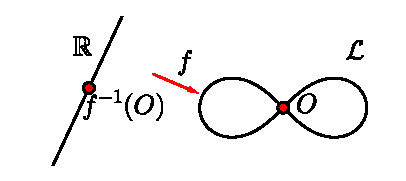
\includegraphics[scale = 0.75]{img/lemniscata}
			\caption{Ilustración del argumento intuitivo.}
			\label{cont_img_lemins}
		\end{figure}
		
		\item \begin{figure}[h!]
			\centering
			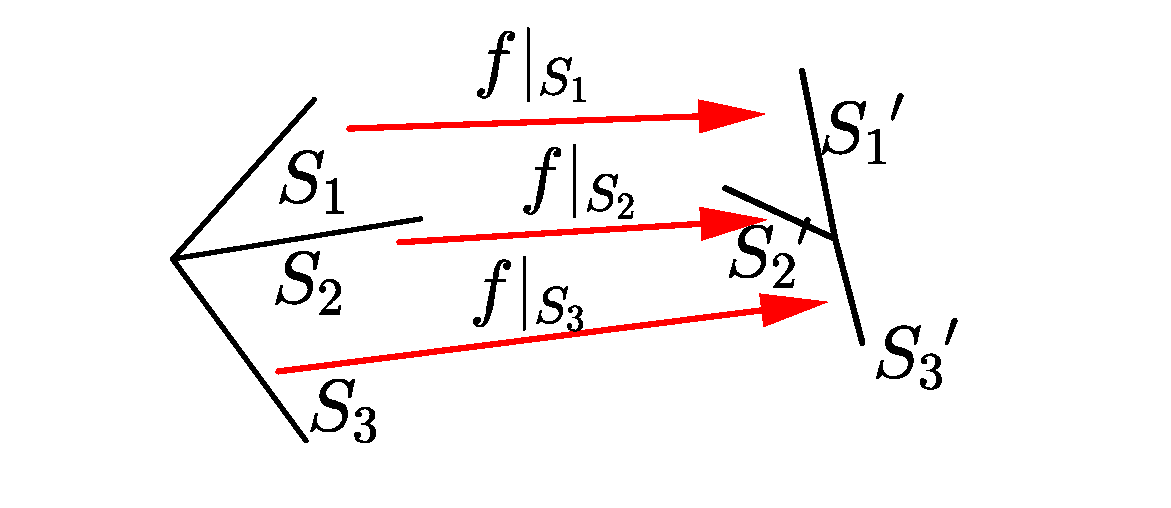
\includegraphics[scale = 0.3]{img/segmentos}
			\caption{Ilustración del homeomorfismo.}
			\label{cont_img_sementos}
		\end{figure}
		
		Sea $\X$ un conjunto de $3$ segmentos cualesquiera de $\R^2$ que comparten un punto extremo e $\Y$ otro conjunto de $3$ segmentos arbitrarios que comparten otro punto extremo (véase la ilustración \ref{cont_img_sementos}). Si equipamos a ambos conjuntos con la topología relativa inducida por la topología usual de $\R^2$, entonces son homeomorfos.
		
		En efecto, tomando el recubrimiento por cerrados de $\X$ compuesto por cada uno de los segmentos y definiendo un homeomorfismo $f$ que a cada segmento (cerrado del recubrimiento de $\X$) le haga corresponder otro segmento de $\Y$ (sin repetir). Tenemos, por la proposición \ref{cont_prop_caracterizacion} que $\X$ e $\Y$ son homeomorfos (así de paso vemos que las proposiciones sirven para algo).
		
		Dicho homeomorfismo $f$ será la \tbi{interpolación lineal} que definimos como
		\begin{equation}
		\label{interpolacion}
			\begin{array}{cc}
			f_{ab}:&[0,1]\to\R^2\\
			& t\mapsto ta+(1-t)b
			\end{array}
		\end{equation}
		Que es un homeomorfismo (¡compruébese!) que transforma el intervalo $[0,1]$ en el segmento de $\R^2$ determinado por los puntos $a,b\in\R^2$, al que denotamos por $[a,b]$ con cierto abuso de notación.
		
		Para conseguir un homeomorfismo entre dos segmentos $[a,b]$ y $[c,d]$ cualesquiera basta seguir el siguiente diagrama.
		\[\xymatrix{[0,1]\ar[r]^{f_{ab}}\ar[d]_{f_{cd}}&[a,b]\\
			[c,d]\ar[ru]_{f_{ab}\circ f^{-1}_{cd}}
			}\]
	\end{enumerate}
	Con esto ya tenemos suficiente artillería para resolver gran cantidad de problemas.
\end{exa}

Una vez definido el concepto de homeomorfismo y vista a través de los ejemplos su gran fuerza, vamos a pasar al concepto de homeomorfismo local, el cual, a pesar de ser una relación más débil que la que proporciona el homeomorfismo, también será muy utilizado.

\begin{defi}[Homeomorfismo local]
	\label{cont_def_homeomorfismoLocal}
	Sea $f:X\rightarrow Y$ aplicación entre espacios topológicos y $x_0\in X$. Se dice que $f$ es \tbi[homeomorfismo!local]{homeomorfismo local} en $x_0$ si $x_0$ tiene un entorno abierto $U_{x_0}$ tal que $f(U_{x_0})$ es entorno abierto de $f(x_0)$ en $Y$ y se tiene que $f|_{U_{x_0}}:U_{x_0}\rightarrow f(U_{x_0})$ es homeomorfismo.
\end{defi}

De esta definición se desprende que todo un homeomorfismo entre dos espacios es en un homeomorfismo local en todos sus puntos. Este resultado resulta evidente, pero su contrarreciproco (no homeomorfo local implica no homeomorfo) nos puede resultar enormemente útil ya que es mucho más sencillo estudiar  el homeomorfismo local al global.

Vemos ahora, a modo de ejemplo que la esfera $\esfera^2:=\{x\in\R^3\midc\norm{x}=1\}$ es localmente homeomorfa al plano $\R^2$.

\begin{exa}[Esfera y plano]
	\label{cont_exa_homeomorfismoLocal}
	Vamos a contruir un homeomorfismo local entre la esfera y el plano.
	
	Resulta de interés destacar que no es necesario que la aplicación sea la misma en todo el espacio, sino que podemos tomar una distinta para cada punto del espacio.
	
	En efecto, sea $p:=(x_0,y_0,z_0)\in\esfera^2$ con $z_0\not=0$, entonces, dado un entorno abierto de $p$ que no corta al ecuador de la esfera y queda contenido en el hemisferio de $p$, definimos la aplicación
	\[\begin{array}{cc}
	f(x,y,z):=(x,y) \qquad& f^{-1}(x,y):=(x,y,\frac{z_0}{\abs{z_0}}\sqrt{1-x^2-y^2})
	\end{array}\]
	que es homeomorfismo local (¡compruébese!).
	
	Análogamente, si tomamos un $p':=(x_1,y_1,0)\in\esfera^2$ con $x_1>0$, dado un entorno abierto de $p'$ con todos los puntos con primera coordenada positiva definimos el siguiente homeomorfismo local (¡compruébese!)
	\[\begin{array}{cc}
	f(x,y,z):=(y,z) \qquad& f^{-1}(y,z):=(\sqrt{1-y^2-z^2},y,z)
	\end{array}\]
	Nótese que aún quedan puntos de la esfera por tratar (se dejan como ejercicio).
\end{exa}

Una vez vistas ambas definiciones pasamos a ver una serie de propiedades y observaciones propias de los homeomorfismos (globales), pero que también nos valdrán para la restricción homeomorfa de los locales (dado que en ella por definición la aplicación es homeomorfa).
\label{etop_obs_homeomorfismo}
\begin{obs}[Propiedades de los homeomorfismos]\
	\begin{enumerate}
		\item 
		Sea $f:X\rightarrow Y$ aplicación biyectiva.
		
		Que $f$ sea continua es equivalente a que si $U\in Y$ es abierto, $f^{-1}(U)$ también lo será. Del mismo modo, es equivalente a que si $F\in Y$ es cerrado, $f^{-1}(F)$ también lo será.
		
		Igualmente, que $f^{-1}$ sea continua es equivalente a que si $F\in X$ es cerrado, entonces $f(F)$ es cerrado, asimismo si $U\in X$ es abierto, $f(U)$ también lo será.
		
		Vemos como si se verifican ambas (la continuidad de $f$ y de su inversa) será homeomorfismo, de modo que $f$ es homeomorfismo si y solo si es continua, biyectiva y transforma abiertos en abiertos por imágenes directas.
		
		\item
		Una aplicación $f$ no necesariamente biyectiva se dice \tbi[aplicación!abierta]{abierta} cuando la imagen de abiertos es un abierto (es decir, cuando $f(U)$ es abierta si $U$ es abierto).
		
		Análogamente, una aplicación $f$ no necesariamente biyectiva se llama \tbi[aplicación!cerrada]{cerrada} cuando la imagen de cerrados es un cerrado (es decir, cuando $f(F)$ es cerrado si $F$ es cerrado).
		
		Dejamos como ejercicio al lector ver que si una es aplicación no es abierta no tiene por qué ser cerrada (y viceversa) y que si una aplicación es abierta y cerrada no tiene por qué ser biyectiva.\qedhere
		\end{enumerate}
\end{obs}

		
	\appendix
	%A partir de aquí los capítulos son apéndices.
	
	%-----Archivos Temporales----- 
	%Cosas Pendientes de Álvaro García Tenorio
	%Cosas Pendientes de Iván Prada Cazalla
\section{Examen Septiembre 2007}
\subsubsection{Problema 1}
Se considera en el plano $\R^2$ los \ti{triángulos semiabiertos} de vértice $(a,b)\in \R^2$ y anchura $\varepsilon > 0$ definidos por:
\begin{equation}
	U = \{(x,y) \in \R^2 \tq x-y \geq a - b, x + y \geq a + b, a \leq x \le a + \varepsilon\}
\end{equation}
y equipamos $\R^2$ con la topología $\T$ que tiene todos esos triángulos por bases de abiertos.
\begin{enumerate}
	\item Calcular la adherencia (en $\T$) de un triángulo semiabierto $\U$.
	\item Estudiar si $(\R^2,\T)$ es Lindelöf. ¿Y es localmente compacto?
	\item Demostrar que los únicos conjuntos conexos para esta topología son los puntos.
	\item Existe alguna topología $\T_1$ en $\R$ tal que $\T$ sea la topología del producto $\T_1 \times \T_1$? ¿Y tal que $(\R^2,\T)$ sea homeomorfo a $(\R^2,\T_1 \times \T_1)$?
	{\large a}
\end{enumerate}
\begin{proof}
	Lo primero de todo, vamos a hacernos una idea de como son estos abiertos:
	
	Por la descripción de estos abiertos, vemos que los abiertos son de la siguiente manera:
	\begin{figure}[h!]
		\centering
		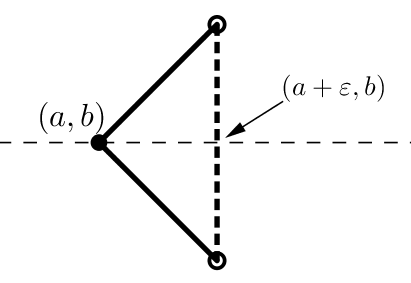
\includegraphics[scale = 1.5]{img/ExamenSeptiembre2017/Abiertosimg}
	\end{figure}
	Estos serán los abiertos de nuestra base de abiertos de la topología $\T$.
	Algo muy importante y que se resaltará siempre es que solo hemos de responder a lo que se nos pide. En este caso ya se nos dice que es una base de la topología, por lo tanto no tenemos que comprobarlo ni nada por el estilo. Podemos jugar con este hecho desde el principio, ya que nos lo da el enunciado.
	\begin{enumerate}
		\item Vamos a hacer una serie de apreciaciones antes de proceder a la resolución de este apartado. Hemos de observar que $\T_u \varsubsetneq \T$. Esto implica que la topología $\T$ es más fina que la usual. Esto se desprende de que cualquier abierto de de la usual contiene un abierto de $\T$, y que esta contención es estricta de que los triángulos no son abiertos en la usual.(La otra contención no se da ya que no podemos meter abiertos de la usual para ciertos puntos del triángulo, como por ejemplo el vértice).
		
		Vamos a calcular entonces la \tb{adherencia de un triángulo semiabierto}. La primera idea intuitiva que nos surge es añadirle al abierto el segmento vertical con los extremos incluidos que une los dos vértices del triángulo.
		
		\begin{figure}[h!]
			\centering
			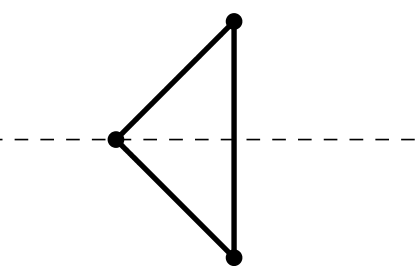
\includegraphics[scale = 1.5]{img/ExamenSeptiembre2017/Abiertosadherencia1img}
		\end{figure}
	
		Estos son cerrados en la topología usual, $\implies$ $\U \subset \adher{U}^{usual}$, luego  $\U \subset \adher{U}^{usual} \subset \adher{U}$.
		Ahora vamos a ver si los puntos que hemos añadido son adherentes. A esto respondemos que no (si llamamos $r$ al segmento citado), ya que $\forall p \in r , \exists V$ entorno de $p \tq \V \cap \U = \emptyset$.
		
		\begin{figure}[h!]
			\centering
			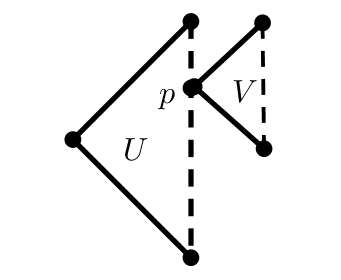
\includegraphics[scale = 1.5]{img/ExamenSeptiembre2017/Abiertosadherencia2img}
		\end{figure}
		
		Por lo tanto la adherencia de $\U$ en esta topología es el propio $\U$, ya que como hemos visto, los puntos de ese segmento no son adherentes.
		
		Si lo hubieramos visto comprobando ``uno a uno" todos los puntos habría que decir además que los puntos de fuera del triángulo no son adherentes ya que existe un abierto en la usual que contiene un triángulo (que es entorno que no corta al conjunto).
		
		Luego  $\adher{\U} = \U$ , lo que implica además que es una base de abiertos y cerrados simultáneamente.
		
		\item Veamos si el espacio topológico es \tb{Lindelöf} \ref{lindel} con esta topología.
		
		Lo primero que tenemos que intentar hacer es ver si hay subespacios especiales (por ejemplo rectas verticales).
		
		Tomamos la recta vertical $r$, subespacio de nuestro espacio topológico con la topología relativa. Si lo cortamos con los abiertos relativos, observamos que $p = r \cap \U^{abierto\ rel.\ en\ r} \implies \T|_r$ es la topología discreta $\implies$ No es II axioma por ser recta con topología discreta $\implies r= \cup_{p\in r}\{p\}$.
		
		Por lo tanto $\T$ no puede ser II axioma, ya que esta es una propiedad hereditaria. Además, $\T$ tampoco es Lindelöf ya que esta es una propiedad hereditaria para cerrados. Como $r$ es cerrado, $\T$ tampoco es Lindelöf.
		
		Para comprobar si es \tb{localmente compacto} procederemos del siguiente modo. Nos hacemos la pregunta, ¿existirá algún entorno compacto?.Supongamos que existe algún entorno compacto $\K^p$. $\exists \K^p \supset \U = \adher{U} \implies \U$ compacto. Nos centraremos en ello.
		Si la respuesta fuera negativa, si encuentro un $\L^{cerrado} \subset \U$ que no es compacto habremos terminado.
		Si tomamos un segmento con los extremos contenidos, vertical, y contenido en un triángulo al que llamaremos $\mathcal{I}$. Si $\exists \K^p \supset \U \supset \mathcal{I}$, la topología de este segmento es la discreta por ser un subespacio de el $r$ que tomamos antes. Además es cerrado en la topología usual. Por lo tanto, $\T|_\mathcal{I}$ es la topología discreta $\implies$ no es compacto (no hay un subrecubrimiento finito), luego hemos terminado ya que al $\mathcal{I}$ no ser compacto no puede existir el supuesto compacto que supusimos.
		\item Veamos si es totalmente disconexo.
		
		Como se vió en resultados teóricos, si un espacio tiene una base \ti{clopen} y es $T_0$ entonces es totalmente disconexo.
		
		SUpongamos que $p,q \in \X, p \neq q\ y\ p,q \in \mathcal{C}$. Veamos que $\mathcal{C}$ no es conexo. Ponemos $\mathcal{C} = (\mathcal{C} \cap \U) \cup (\mathcal{C} \setminus \U)$, sabemos que $\U$ es abierto ambiente ($\U$ es abierto de uno de los puntos que no tiene al otro, que existe por ser $T_0$), y que estas intersecciones son no vacías ya que contienen a los puntos $p$ y $q$. Por lo tanto tenemos dos cerrados que producen la desconexión, y como es para cualquiera dos puntos, el espacio es totalmente disconexo con esta topología. Además se necesita que haya dos puntos distintos.
	
		\item Para ver si algo es topología producto hemos de mirar los productos que lo conforman.
	\end{enumerate}	
\end{proof}
	%Cosas Pendientes de Manuel Navarro García

\textbf{Número 1.1.} Sea $X$ un conjunto, y $\T_{\text{CF}}$ la familia de todos los subconjuntos de $X$ cuyo complementario es finito, más el conjunto vacío. Probar que $\T_{\text{CF}}$ es una topología en $X$. Esta topología se llama, por razones evidentes, \textit{topología de los complementarios finitos}. ?`Qué topología obtenemos si $X$ es un conjunto finito?  \\

A partir del enunciado se deduce que los abiertos de esta topología son los elementos de la colección 

\[\T_{\text{CF}}= \{U \subset X : U= \emptyset \text{ o } X \backslash U\equiv U^c \text{ es finito}\}.\]

Veamos que efectivamente $\T_{\text{CF}}$ es una topología al verificar las condiciones necesarias. 

\begin{itemize}
\item En primer lugar, el vacío pertenece a esta por definición. Además, el complementario del total $X$ (el vacío) es finito, luego $X$ también pertenece a $\T_{\text{CF}}$. 

\item Por otro lado, sea $\{U_\alpha\}_{\alpha \in I}$ para un cierto conjunto de índices $I$ una colección arbitraria de elementos de $\T_{\text{CF}}$, teniéndose que 

\[X \backslash \bigcup_{\alpha}U_\alpha = \bigcap_{\alpha} (X\backslash U_\alpha).\]

Pero $X-U_\alpha$ es finito para cada $\alpha \in I$, luego la intersección numerable de ellos también lo será. De este modo, la unión numerable de abiertos de $\T_{\text{CF}}$ pertenece a ella.

\item Por último, consideremos $U_1$ y $U_2$ dos abiertos de $\T_{\text{CF}}$. Analógamente al caso anterior, 

\[X \backslash (U_1 \cap U_2) = \bigcup_{i=1}^2 (X\backslash U_i).\]

Sin embargo, $X \backslash U_i$ es finito para $i\in\{1,2\}$, luego la unión finita de conjuntos finitos es finita.
\end{itemize}

Para finalizar, se nos pregunta qué topología se obtendría en caso de que $X$ fuese un conjunto finito. Si damos por cierta esta suposición, es claro que $\T_{\text{CF}}$ coincide con la topología discreta, ya que el complementario de todo conjunto es finito. \\

A pesar de haber terminado con lo requerido del ejercicio, podemos ir más allá estudiando más a fondo esta topología. Para comenzar, nótese que si $X$ es numerable trivialmente el conjunto es separable y primer y segundo axioma de numerabilidad. El caso en el que $X$ no es numerable ya no es tan sencillo. Vayamos por partes.

\begin{itemize}
\item $X$ es separable. Es más, todo conjunto numerable es denso en $X$. En efecto, supongamos que existiese un conjunto $A \subset X$ numerable pero que no es denso en $X$. Esto implica que existe un abierto $B\in \T_{\text{CF}}$ tal que $B\cap A = \emptyset$. De este modo, 

\[(X\backslash B)\cup (X\backslash A)=X.\]

Pero los conjuntos del primer miembro son finitos, y la unión de finitos es finita, lo que conllevaría a que $X$ también lo sea. Esto nos conduce a la  contradicción buscada. 

\item $X$ no es primer axioma de numerabilidad, lo que implica que tampoco es segundo. Para corroborar esto, comprobemos que para cada punto $a\in X$ no existe una base de entornos abiertos numerable centrada en $a$. Razonaremos de nuevo por reducción al absurdo. \\

Supongamos que sí que existe esa base y sea esta 

\[\mathcal{U}^a=\{V_k \in\T_{\text{CF}}: k \geq 1\}.\]

La intersección 

\[\left(\bigcap_{k\geq 1} V_k\right)\backslash \{a\}\]

es no vacía puesto que, al tomar los complementarios y aplicar las leyes de De Morgan se tiene que 

\[X \backslash \left(\bigcap_{k\geq 1} V_k\right)= \left(\bigcup_{k\geq 1} X \backslash V_k\right), \]

y esta unión es numerable ya que $X \backslash V_k$ es finito (recordemos que $V_k \in \T_{\text{CF}}$). Al ser $X$ no numerable y 

\[X= \left(\bigcap_{k\geq 1} V_k\right) \cup \left(\bigcup_{k\geq 1} X\backslash V_k\right),\]

la intersección anterior ha de ser no numerable. \\

Tomemos ahora un punto cualquiera $b$ de esta intersección con la condición de que sea distinto de $a$ y consideremos el entorno abierto de $a$ dado por $W:=X\backslash \{b\}$. Claramente, $a\in W$ y es abierto puesto que su complementario es finito.  De forma evidente la condición $V_k \subset W$ no se verifica para ningún $k$ ya que $b\in V_k$ para todo $k$. Esto verifica que $\mathcal{U}^a$ no puede ser base, concluyendo así que cuando $X$ no es numerable $\T_{\text{CF}}$ no es primer axioma de numerabilidad.

\item $X$ es compacto. En efecto, supongamos que $\{V_k : k \geq 1\}$ es un recubrimiento por abiertos de $X$ y tomemos un $V_{k_0}$ arbitrario. Como este abierto pertenece a $\T_{\text{CF}}$ su complementario es finito, luego 

\[X \backslash V_{k_0} := \{x_1, \ldots, x_r\}\]

con $x_j \in X$ y $j=\{1,\ldots, r\}$ tales que $x_j\in V_{k_j}$ para cierto $k_j$, pues la unión de $V_k$ recubre $X$ según lo hemos definido. De este modo, podemos tomar $X$ como la unión de $V_{k_0}$ con los $V_{k_j}$ que contienen a los puntos $x_j$, esto es,

\[X=\bigcup_{j=0}^r V_{k_j},\]

lo que prueba que $X$ es compacto. 

\item $X$ es conexo. Un modo de probar esto es comprobar que no existen conjuntos abiertos y cerrados simultáneamente. En caso de que esto ocurriese, lo que quiere decir que $A\in \T_{\text{CF}}$ y $X\backslash A \in \T_{\text{CF}}$, se tiene que $X \backslash A$ y $X\backslash (X\backslash A)=A$ son finitos, luego

\[X=A \cup (X\backslash A)\]

sería finito, y esto contradice que sea no numerable. 
\end{itemize}

	%Cosas Pendientes de Álvaro Rodríguez García

%%%%%%%%%%
% Día 28/2
%%%%%%%%%%

% Después del primer cacho de imágenes directas
	%Cosas Pendientes de Clara Rodríguez Núñez
	
	%-----Mierdas Varias-----
	%Basurero donde se ponen cosas que no se sabe muy bien donde poner.
	
	\printindex[general]
	\printindex[topologias]
\end{document}